\documentclass[11pt]{amsart}
\usepackage{amssymb,amsmath,graphicx,booktabs,longtable}
\usepackage[margin=1in]{geometry}\usepackage[hidelinks]{hyperref}
\newtheorem{theorem}{Theorem}[section]\newtheorem{lemma}[theorem]{Lemma}
\newtheorem{proposition}[theorem]{Proposition}\newtheorem{corollary}[theorem]{Corollary}
\theoremstyle{definition}\newtheorem{definition}[theorem]{Definition}
\theoremstyle{remark}\newtheorem{remark}[theorem]{Remark}
\title{Every two-colouring of the plane contains a monochromatic $T(1,3,4)$}
\author{Alina Yan}\date{October 2026}
\begin{document}
\begin{abstract}
We prove that every red--blue colouring of the Euclidean plane contains three collinear points of one colour
with consecutive distances $1$ and $3$. The argument works on the triangular lattice $\Lambda=\mathbb Z[\omega]$
together with a single rotated copy $q\Lambda$, where $q=\pi/\bar\pi=(3+5\omega)/7$ and $\pi=2+\omega$; the two
lattices share a sublattice of index $7$. Using the structure theorem for $T(1,3,4)$-avoiding colourings of the
triangular lattice from the author's thesis, we show that every lattice line is coloured in runs of exactly four
(Rule A) and that the resulting bands never change their offset step (Rule B). Then any two points at distance $8$
have the same colour, which forces a monochromatic unit triangle.
\end{abstract}
\maketitle

\section{Introduction}
For $a,b,c>0$ write $T(a,b,c)$ for a configuration of three points with pairwise distances $a,b,c$, the degenerate
(collinear) case allowed, and $T(s)=T(s,s,s)$. A colouring \emph{contains} a configuration if some congruent copy is
monochromatic. Erd\H{o}s, Graham, Montgomery, Rothschild, Spencer and Straus~\cite{EGMRSS} initiated the study of
which configurations every two-colouring of the plane must contain. Currier, Moore and Yip~\cite{CMY24} proved that
every two-colouring of the plane contains a monochromatic three-term arithmetic progression, that is, a
monochromatic $T(1,1,2)$, which was an inspiration to this research.

\begin{theorem}\label{thm:main}
Every two-colouring of $\mathbb R^2$ contains a monochromatic $T(1,3,4)$.
\end{theorem}

Scaling gives a monochromatic $T(a,3a,4a)$ for every $a>0$. The proof has four steps.
\begin{enumerate}
\item \emph{Rule A} (Section~\ref{sec:A}): along the long direction of any unit triangular lattice, monochromatic runs
have length exactly four.
\item \emph{Bands} (Section~\ref{sec:bands}): every unit triangular lattice is coloured in bands of width four, whose
offsets advance by $4$ or $5$ from row to row.
\item \emph{Rule B} (Section~\ref{sec:B}): these steps never change between $4$ and $5$.
\item \emph{Distance eight} (Section~\ref{sec:end}): any two points at distance $8$ have the same colour, so every unit
equilateral triangle is monochromatic.
\end{enumerate}
The structural input is the description of $T(1,3,4)$-avoiding colourings of the triangular lattice from the
author's thesis~\cite{Yan}, and the idea of overlapping a lattice with a rotated copy proposed in its conclusion.
Both finite arguments use only the base lattice and one rotation.

\section{Preliminaries}
Let $\omega=e^{i\pi/3}$, so $\omega^2=\omega-1$ and $\bar\omega=1-\omega$, and $\Lambda=\mathbb Z+\mathbb Z\omega$ with
$|a+b\omega|^2=a^2+ab+b^2$. A \emph{unit triangular lattice} is a set $z_0+u\Lambda$ with $|u|=1$; its three
\emph{directions} are $u,u\omega,u\omega^2$, and its \emph{rows} in a direction are the lines parallel to it.

\paragraph{The rotation.} Let $\pi=2+\omega$, a prime of norm $7$, and
\[
q=\frac{\pi}{\bar\pi}=\frac{\pi^2}{7}=\frac{3+5\omega}{7},\qquad |q|=1 .
\]
Since $\pi=q\bar\pi$, the sublattice $\pi\Lambda$ of index $7$ lies in both $\Lambda$ and $q\Lambda$
(Figure~\ref{fig:overlap}). Every point of $\Lambda\cup q\Lambda$ is $[a,b]:=(a+b\omega)/7$ with $a,b\in\mathbb Z$; it lies
in $\Lambda$ iff $7\mid a,b$, and in $q\Lambda$ iff $49\mid 8a+5b$ and $49\mid 3b-5a$. Points of $q\Lambda$ are written
$q(m+n\omega)$. The mirror rotation $(5+3\omega)/7$ is the image of $q$ under reflection in the real axis, up to a
unit, and could replace $q$ throughout after reflecting every picture.

\begin{figure}[h]\centering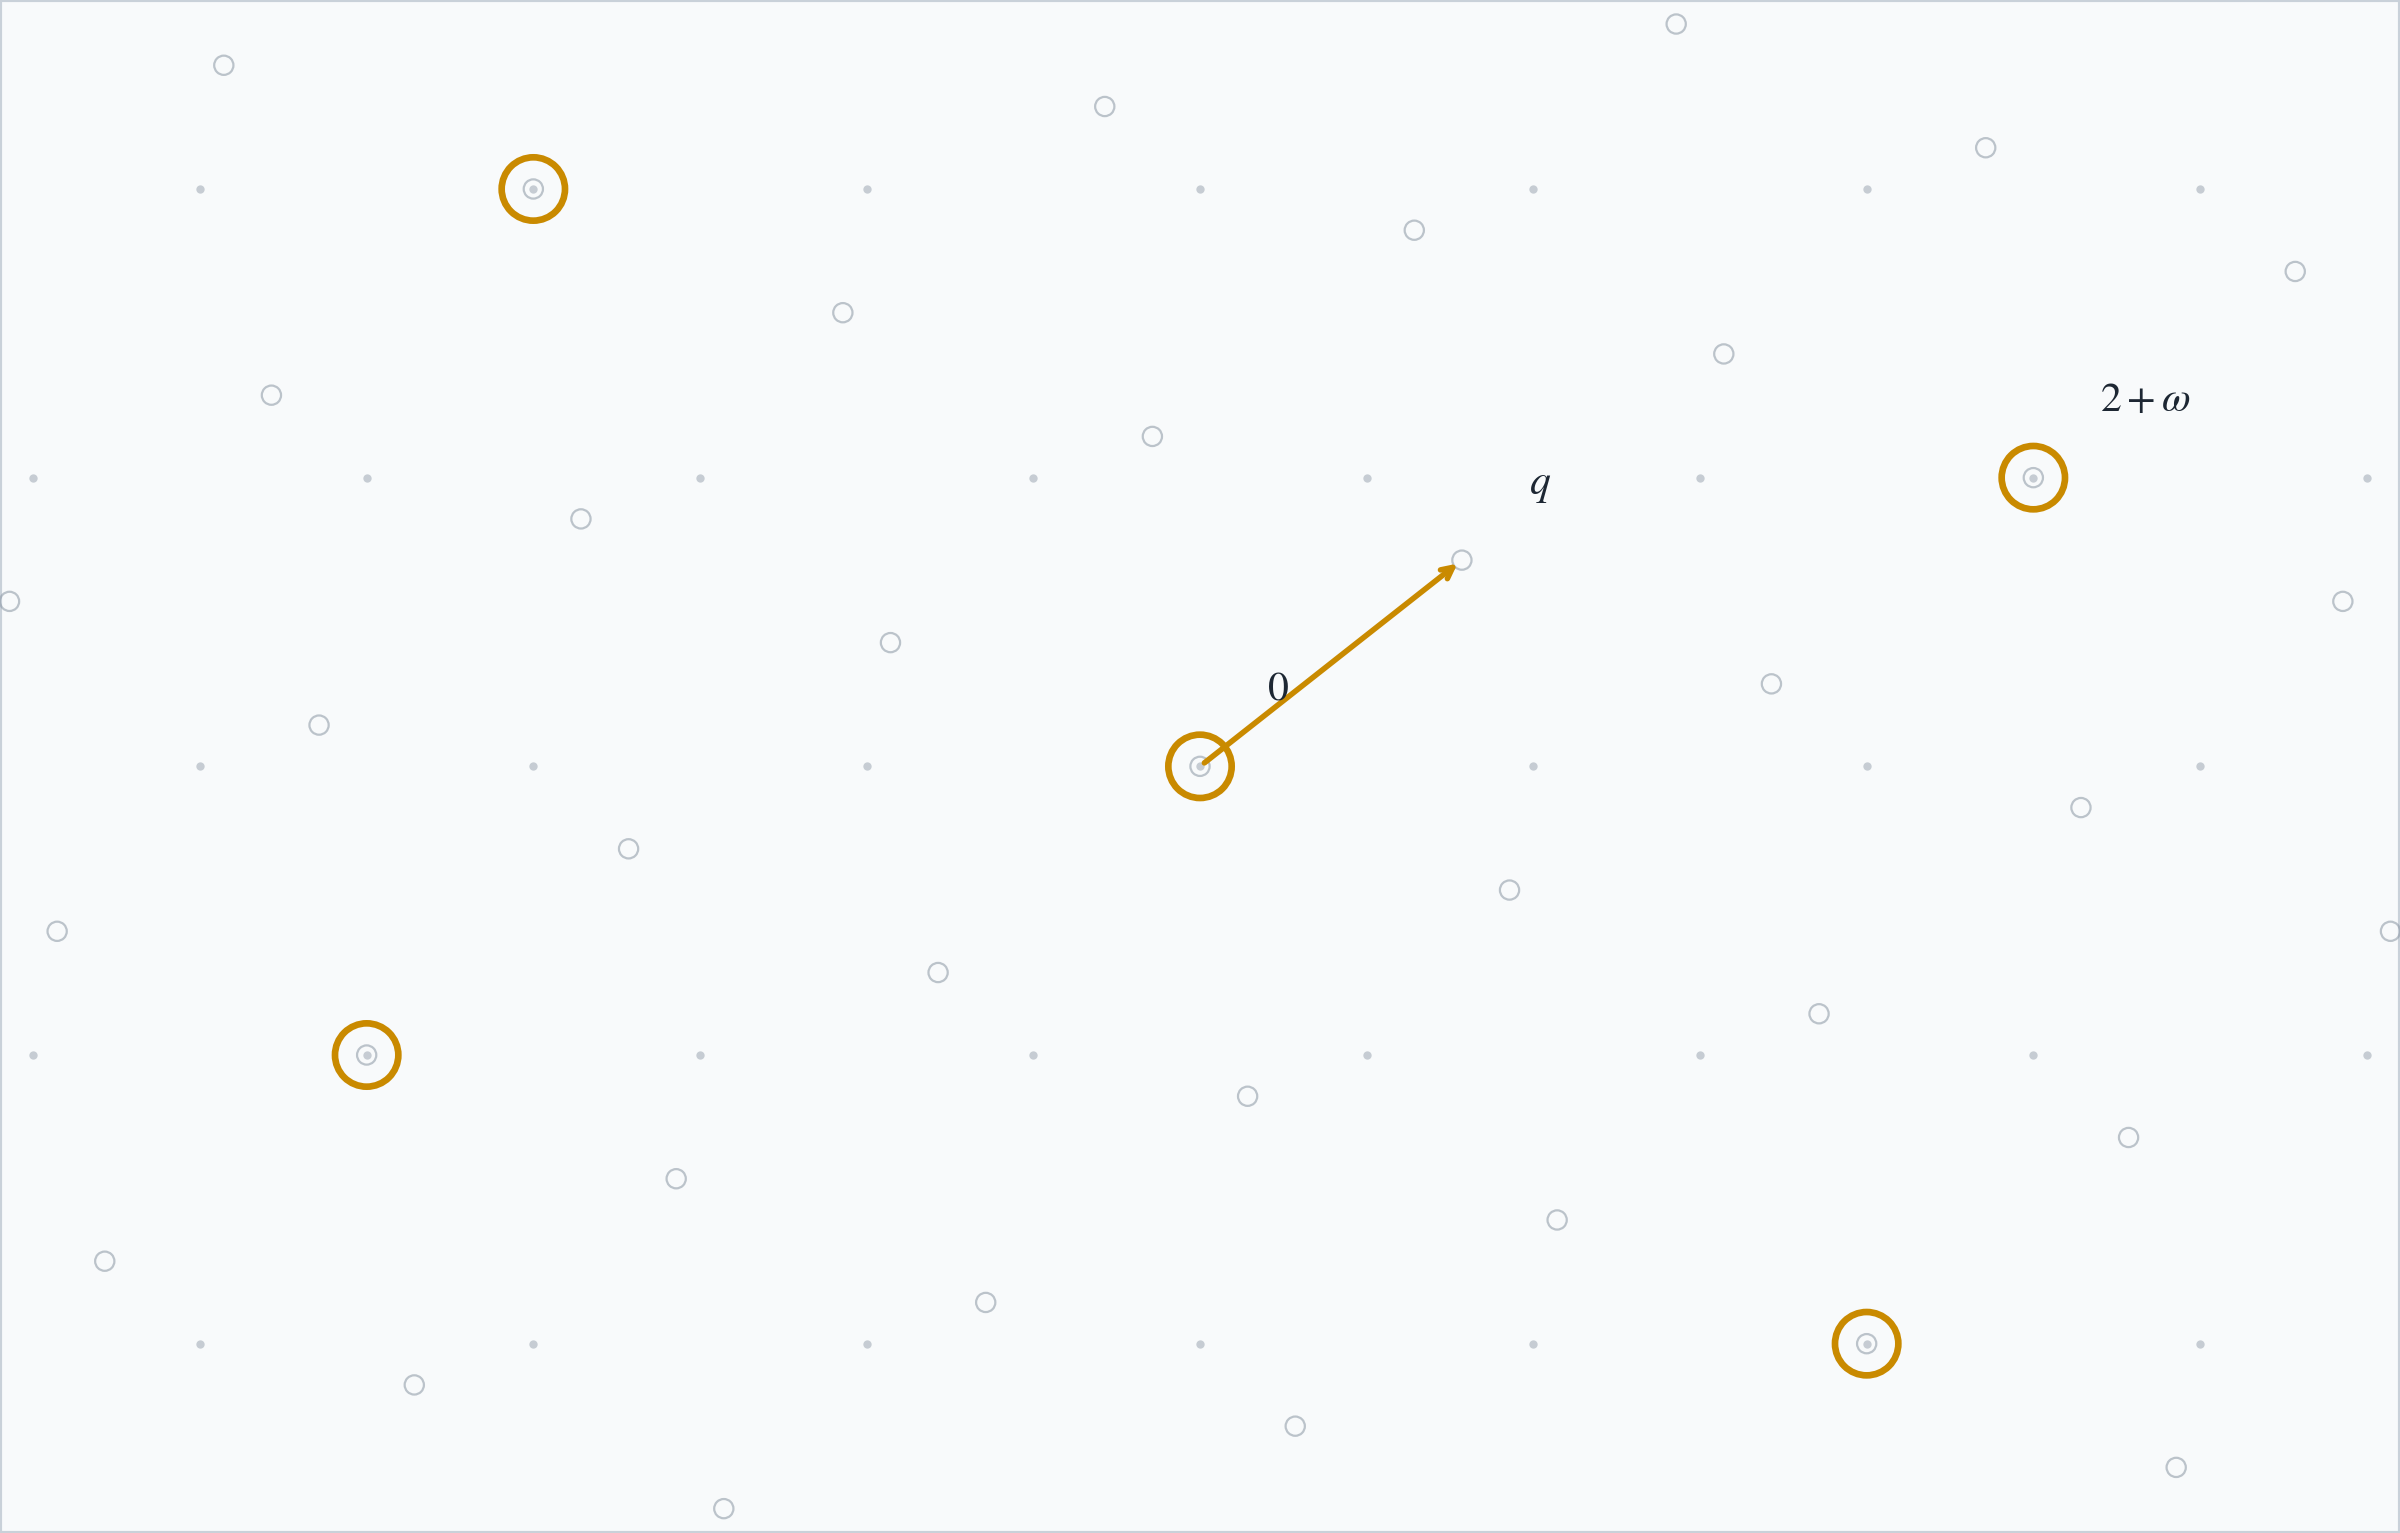
\includegraphics[width=\textwidth]{figures/overlap.png}
\caption{$\Lambda$ (grey dots) and $q\Lambda$ (grey circles); the ringed points form the common sublattice $\pi\Lambda$, which contains $0$, $q\bar\pi=2+\omega$ and its multiples.}\label{fig:overlap}
\end{figure}

\paragraph{Forbidden triangles.} A two-colouring of the plane is \emph{admissible} if it contains no monochromatic
$T(1,3,4)$; we assume one is given and derive a contradiction. The following is the eight-point argument
of~\cite{EGMRSS}.

\begin{lemma}[bridge]\label{lem:bridge}
An admissible colouring contains no monochromatic $T(1)$, $T(3)$ or $T(4)$.
\end{lemma}
\begin{proof}
With $c=1$, $b=4$ put $A=0$, $B=c$, $C=b$, $D=c-c\omega$, $E=b+(c-b)\omega$, $F=b-b\omega$, $G=c-b\omega$,
$H=b+c-b\omega$. The triples $ABC,ADF,BDG,CEF,FGH,BEH$ are copies of $T(1,3,4)$, and $ABD,ACF,BCE,DFG,EFH,BGH$ are
equilateral of sides $1,4,3,3,1,4$; in particular $ABD$, $BCE$, $ACF$ have sides $1$, $3$, $4$. Assume there is no
monochromatic $T(1,3,4)$, so each of the six collinear triples contains both colours. If $A,B,D$ are red, then
$ABC,ADF,BDG$ give $C,F,G$ blue, then $CEF,FGH$ give $E,H$ red, and $BEH$ is red. If $A,C,F$ are red, then
$ABC,ADF,CEF$ give $B,D,E$ blue, then $BDG,BEH$ give $G,H$ red, and $FGH$ is red. If $B,C,E$ are red, then
$ABC,CEF,BEH$ give $A,F,H$ blue, then $ADF$ gives $D$ red and $BDG$ gives $G$ blue, and $FGH$ is blue. Every
equilateral triangle of side $1$, $3$ or $4$ is congruent to $ABD$, $BCE$ or $ACF$, and exchanging colours covers
blue triangles.
\end{proof}

A \emph{forbidden triangle} is a $T(1)$, $T(3)$, $T(4)$ or $T(1,3,4)$. Every finite argument below uses one rule:
\begin{quote}\textbf{(F)} If two vertices of a forbidden triangle have the same colour, the third has the other colour.\end{quote}

\paragraph{The structure theorem.} We use the following result from the thesis.
\begin{theorem}[{\cite[Theorem 3.13]{Yan}}]\label{thm:313}
In a $T(1,3,4)$-avoiding two-colouring of a unit triangular lattice, one of the three directions, the \emph{long
direction}, has all maximal monochromatic runs of length $3$ or $4$; in each of the other two directions every run
has length $1$ or $2$.
\end{theorem}
The restriction of an admissible colouring to any unit triangular lattice is $T(1,3,4)$-avoiding, so
Theorem~\ref{thm:313} applies to $\Lambda$, to $q\Lambda$, and to all their images under isometries.

\section{Rule A}\label{sec:A}
\begin{theorem}[Rule A]\label{thm:A}
In an admissible colouring, no line of a unit triangular lattice carries a maximal monochromatic run of exactly three
points.
\end{theorem}

\begin{lemma}[the row]\label{lem:row}
If such a run exists then, after an isometry and possibly exchanging colours, $0,1,2$ are red and $-3,-2,-1$ and
$3,4,5$ are blue.
\end{lemma}
\begin{proof}
Normalise the run to $0,1,2$ red with $-1,3$ blue, in a lattice $\Lambda$. A run of length three lies in the long
direction by Theorem~\ref{thm:313}, and runs there have length at least three, so the blue runs through $-1$ and $3$
contain $-3,-2,-1$ and $3,4,5$.
\end{proof}

\begin{lemma}[the boundary]\label{lem:boundary}
In this situation $1-\omega,2-\omega,\omega,1+\omega$ are blue, at least one of $-\omega,3-\omega$ is blue, and at least
one of $-1+\omega,2+\omega$ is blue.
\end{lemma}
\begin{proof}
The unit triangles $\{0,1,1-\omega\}$, $\{1,2,2-\omega\}$, $\{0,1,\omega\}$, $\{1,2,1+\omega\}$ have two red vertices. The
rows $\mathbb Z\pm\omega$ are lines of the long direction, so the blue runs through $1-\omega,2-\omega$ and through
$\omega,1+\omega$ have length at least three.
\end{proof}

\begin{figure}[h]\centering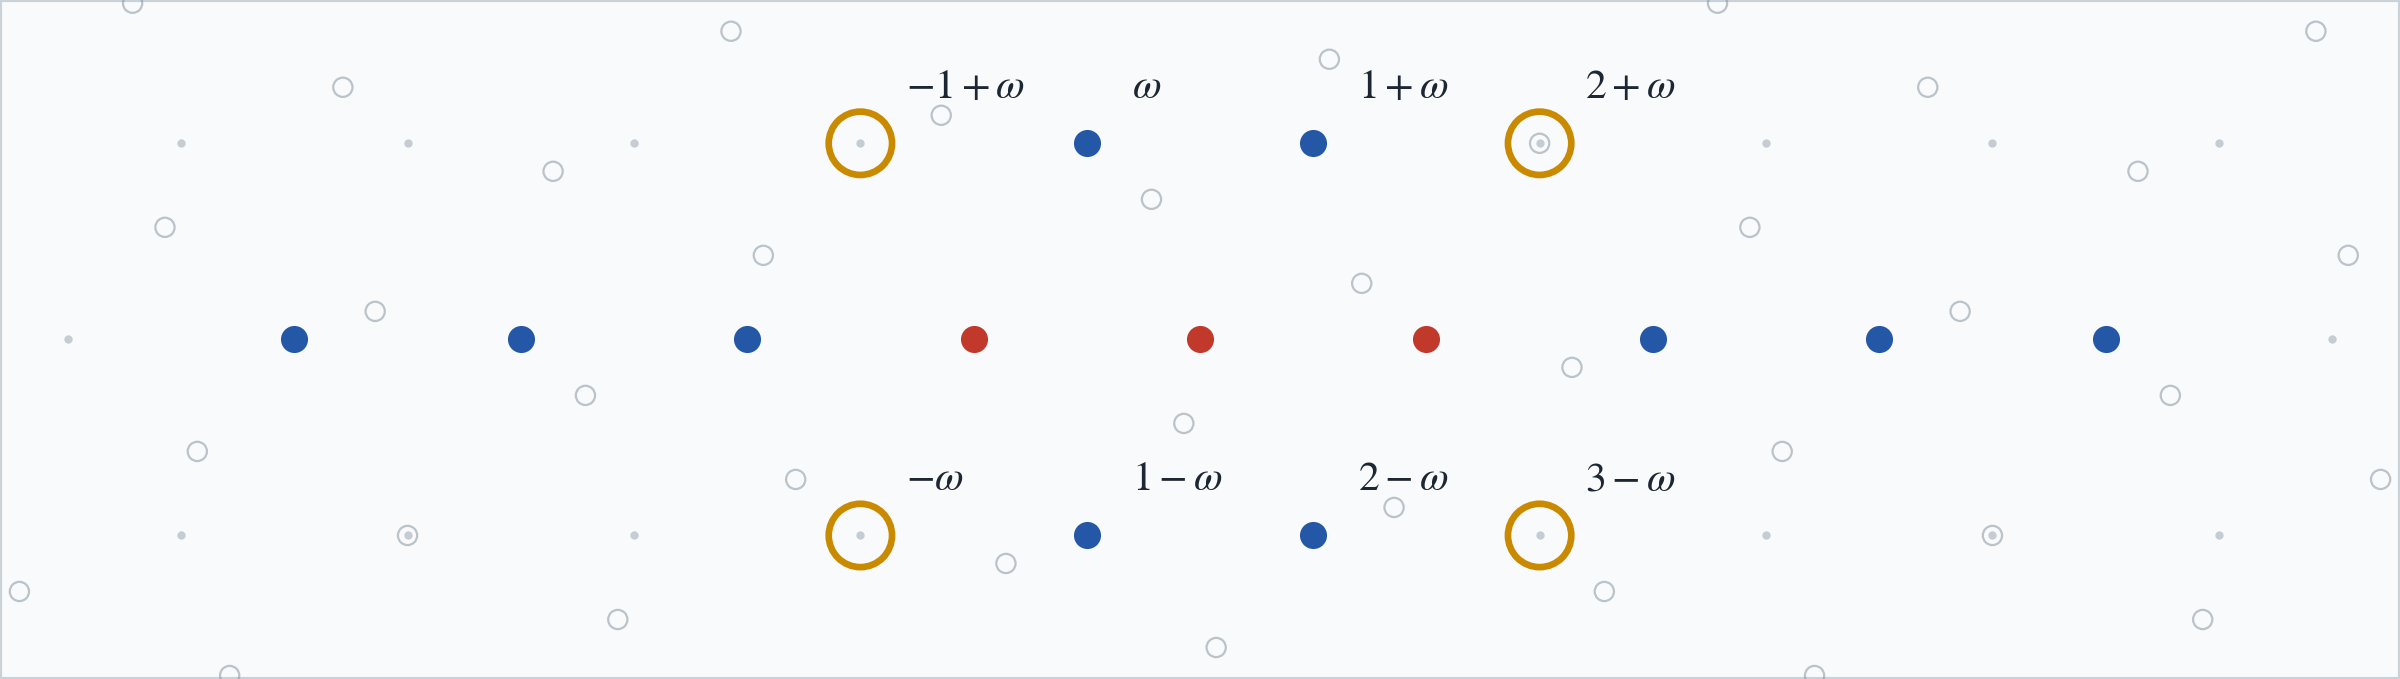
\includegraphics[width=\textwidth]{figures/ruleA_setup.png}
\caption{Rule A: the row $-3,\dots,5$, the four points forced blue by unit triangles, and the four boundary points
(ringed), of which each pair below and above contains a blue point.}\label{fig:Asetup}\end{figure}

\begin{lemma}[symmetries]\label{lem:sym}
The reflections $\tau(z)=\bar z$ and $\sigma(z)=2-\bar z$ preserve the row of Lemma~\ref{lem:row} with its colours.
$\sigma$ swaps $-\omega\leftrightarrow3-\omega$ and $-1+\omega\leftrightarrow2+\omega$; $\tau$ swaps
$-\omega\leftrightarrow-1+\omega$ and $3-\omega\leftrightarrow2+\omega$. If $\chi$ is admissible, so is $\chi\circ\rho$
for every isometry $\rho$.
\end{lemma}
\begin{proof}
Both maps preserve the real axis, $\tau$ pointwise and $\sigma$ as $x\mapsto2-x$, which preserves the colours of
$-3,\dots,5$. For example $\sigma(-\omega)=2-\overline{-\omega}=2-(\omega-1)=3-\omega$.
\end{proof}

\begin{proof}[Proof of Theorem~\ref{thm:A}]
By Lemma~\ref{lem:boundary} the colours of $(-\omega,\,3-\omega,\,-1+\omega,\,2+\omega)$ have a blue point in each pair:
nine possibilities. The group $\{1,\sigma,\tau,\sigma\tau\}$ permutes them in four orbits, of sizes $1,4,2,2$, with
representatives: all four blue; $3-\omega,-1+\omega,2+\omega$ blue; $3-\omega,2+\omega$ blue; $-\omega,2+\omega$ blue.
Replacing $\chi$ by $\chi\circ\rho$ we may assume the boundary is one of these. Each is refuted inside
$\Lambda\cup q\Lambda$ by rule (F), with one case split; the complete deductions are in Appendix~\ref{app:A}.
\end{proof}

\begin{remark}
A second proof uses only $\sigma$: assume $3-\omega$ is blue, then split on the point $q$. If $q$ is red, rule (F)
alone gives a contradiction; if $q$ is blue, one more split finishes. It needs two splits in total but $81$ points
instead of $49$; see Appendix~\ref{app:A2}. In particular $q$ is blue in every such configuration.
\end{remark}

\section{Bands}\label{sec:bands}
Let $h:\mathbb Z/8\to\{\mathrm R,\mathrm B\}$ be red on $0,1,2,3$ and blue on $4,5,6,7$.
\begin{lemma}[bands of width four]\label{lem:bands}
Let $L=z_0+u\Lambda$ be a unit triangular lattice with long direction $u$. There are offsets $s_b\in\mathbb Z/8$ with
\[
\chi\bigl(z_0+u(a+b\omega)\bigr)=h(a+s_b),\qquad s_{b+1}-s_b\in\{4,5\}.
\]
\end{lemma}
\begin{proof}
By Theorem~\ref{thm:313} and Rule A every run in the long direction has length exactly four, so each row is
$a\mapsto h(a+s_b)$. The points $a$, $a+1$, $a+\omega$ form a unit triangle, so under a red run $t,\dots,t+3$ of row $b$
the points $t,t+1,t+2$ of row $b+1$ are blue by (F); hence the blue run of row $b+1$ starts at $t-1$ or $t$, which
says $s_{b+1}\in\{s_b+4,s_b+5\}$.
\end{proof}
\begin{corollary}[four apart]\label{cor:four}
In $L$, points $z$ and $z+4u$ have opposite colours, since $h(x+4)\ne h(x)$.
\end{corollary}
The differences $s_{b+1}-s_b$ are the \emph{steps}; a \emph{turn} is a step of $4$ followed by $5$ or of $5$ followed
by $4$.

\section{Rule B}\label{sec:B}
Fix a row of $L$ in its long direction. The points of the neighbouring rows sit above and below consecutive pairs
of that row, and by (F) every such point under a monochromatic pair has the other colour. This fixes three of every
four points in each neighbouring row; the fourth, above or below a change of colour, is \emph{open}. Open points come
in vertically aligned pairs, one above and one below the row (Figure~\ref{fig:opening}).

\begin{lemma}\label{lem:pair}
The two points of an open pair have the same colour exactly when the two steps at this row form a turn.
\end{lemma}
\begin{proof}
With the row as row $0$ and offset $0$, the point $a+\omega$ lies above the pair $a,a+1$, and $(a+1)-\omega$ lies below
it at the same horizontal position. It is open exactly when $h(a)\neq h(a+1)$, and its colours are $h(a+d_1)$ and
$h(a+1-d_0)$, where $d_0,d_1\in\{4,5\}$ are the steps below and above. For $a=3$ these are $h(3+d_1)$ and $h(4-d_0)$,
which agree iff $d_0\ne d_1$; the case $a=7$ is the same shifted by $4$.
\end{proof}

\begin{figure}[h]\centering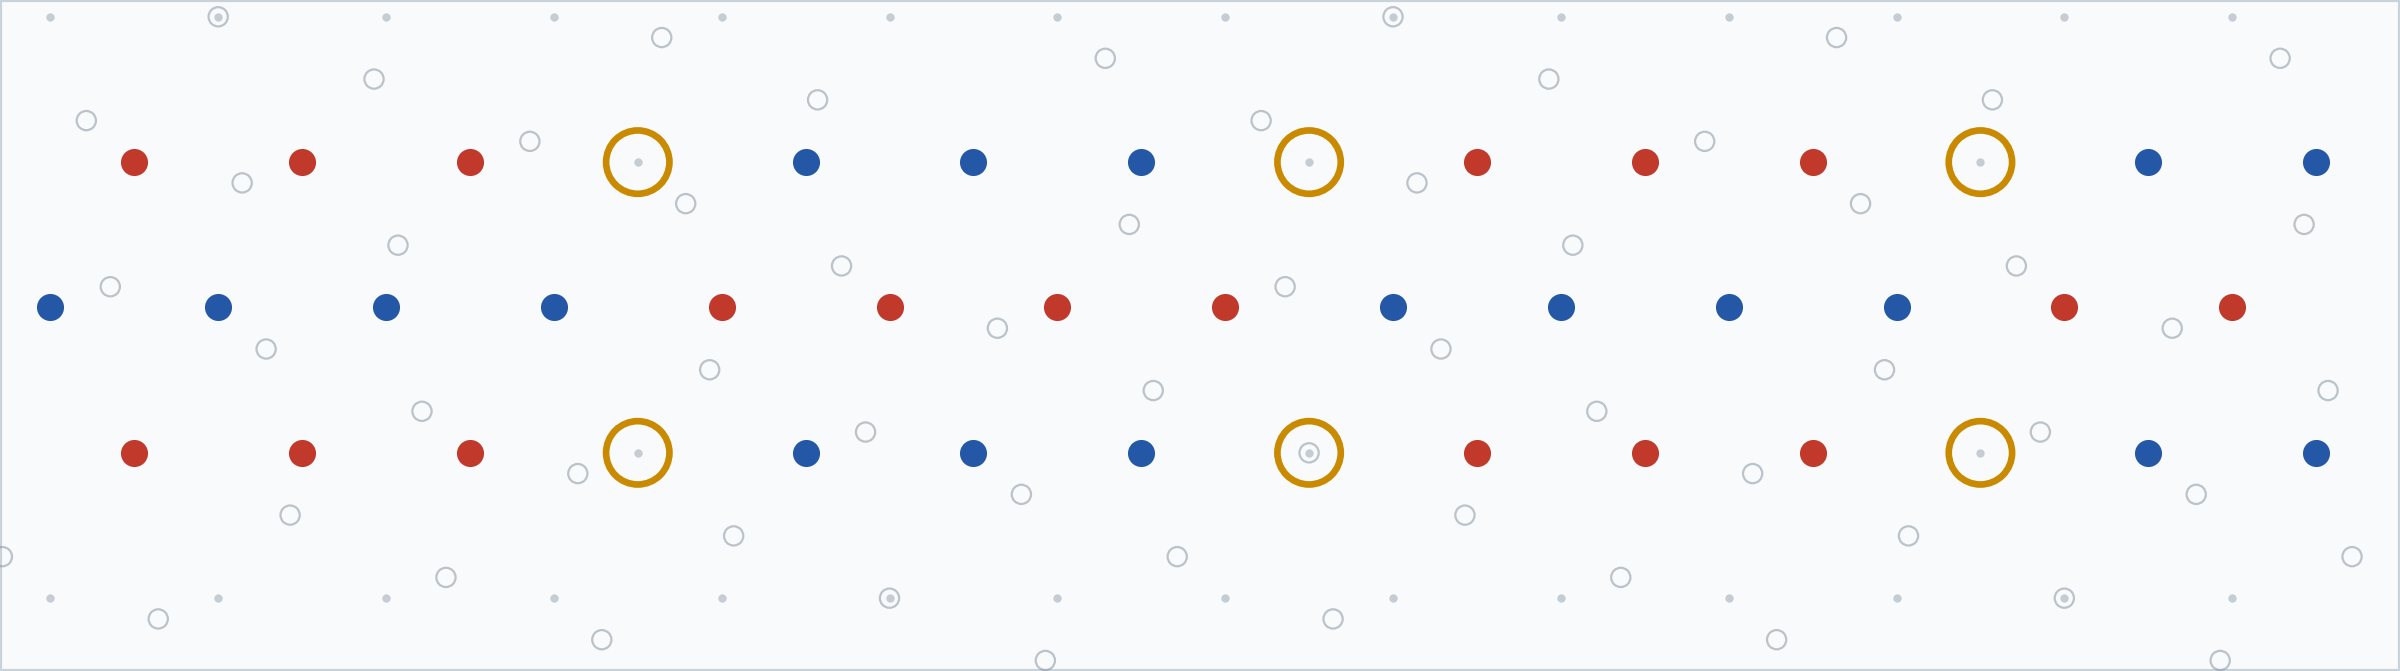
\includegraphics[width=\textwidth]{figures/ruleB_one_row.png}
\caption{One row of the long direction, and the points it forces by unit triangles in the rows above and below.
The open points (ringed) come in vertically aligned pairs.}\label{fig:opening}\end{figure}
\begin{figure}[h]\centering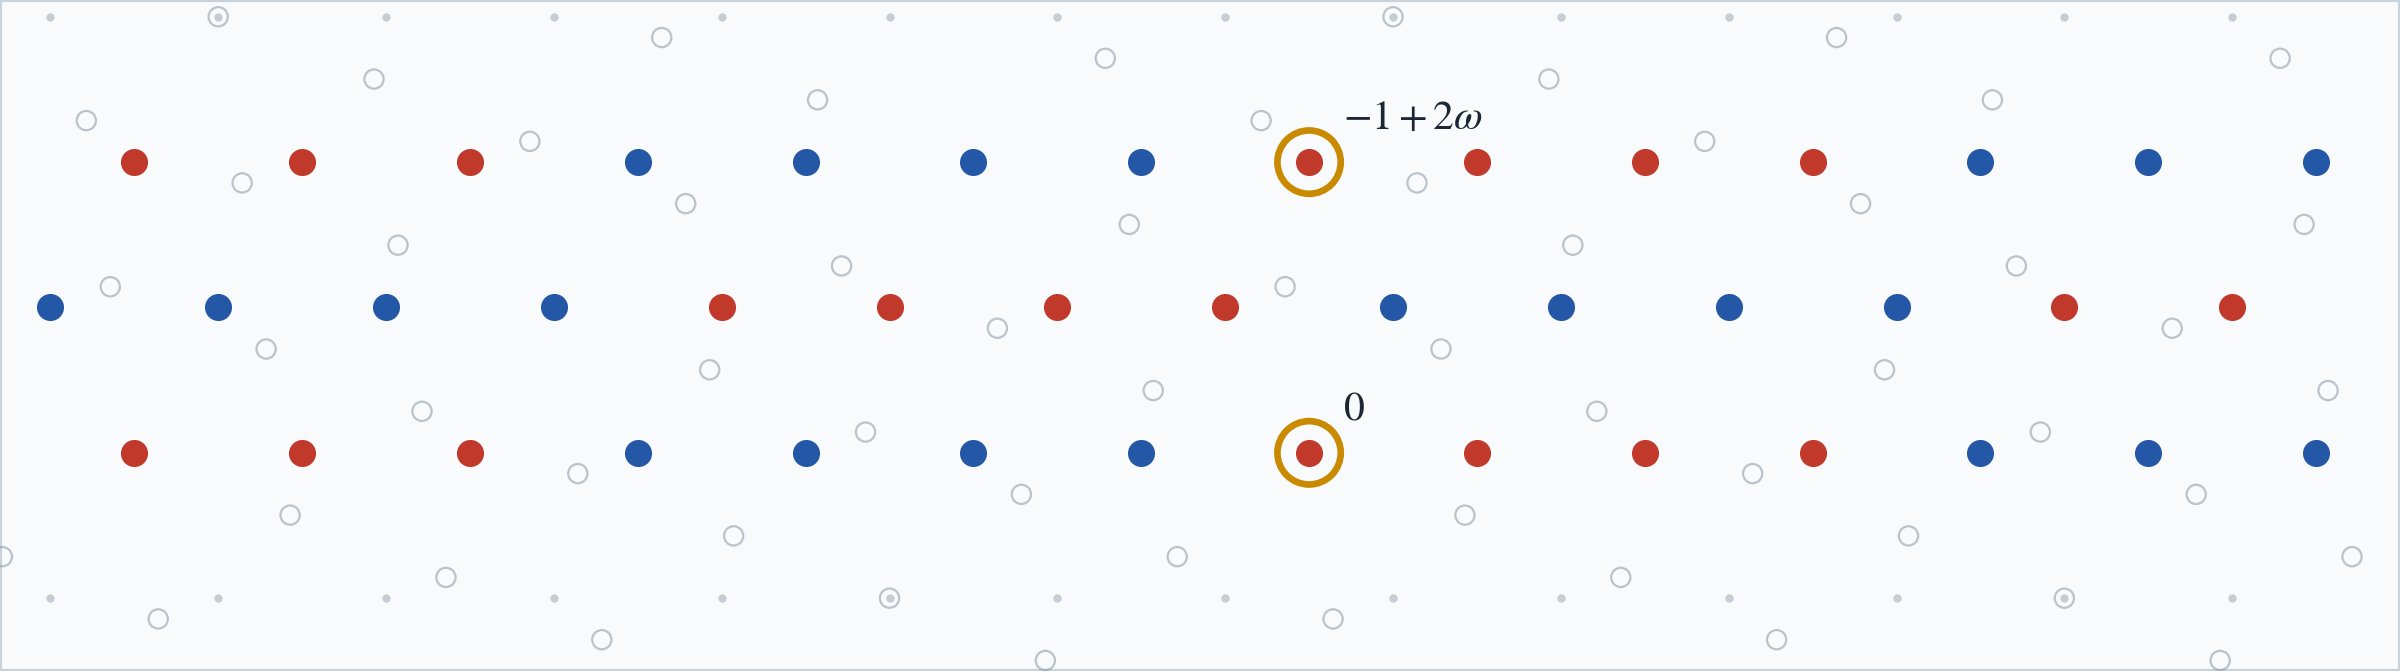
\includegraphics[width=\textwidth]{figures/ruleB_turn.png}
\caption{A same-coloured open pair: here $0$ and $-1+2\omega$ are both red, and rows $0,1,2$ have offsets $0,4,1$,
a turn.}\label{fig:turn}\end{figure}

\begin{theorem}[Rule B]\label{thm:B}
In an admissible colouring no unit triangular lattice has a turn. Equivalently, the two points of every open pair
have different colours.
\end{theorem}
\begin{proof}
Since $h(-x)=h(x+3)$, the half-turn $z\mapsto-z$ replaces $s_b$ by $3-s_{-b}$ and reverses the order of the steps,
so it suffices to exclude a step of $4$ followed by $5$. After an isometry and a translation along the rows, the
lattice is $\Lambda$ with long direction $1$ and offsets $s_0=0$, $s_1=4$, $s_2=1$; rows $0,1,2$ are then fixed. We use
only these three rows, rule (F), and Corollary~\ref{cor:four} applied to $q\Lambda$.

\emph{Common deductions.} Inside $\Lambda$ alone, (F) gives five further colours (Table~\ref{tab:common}).

\begin{table}[h]\caption{Deductions inside $\Lambda$, valid in every case.}\label{tab:common}\vspace{-1ex}
\begin{center}\small\begin{longtable}{rlll}\toprule & point & colour & because\\\midrule\endhead
1 & $-2-\omega$ & red & $T(1)$ with $-3$, $-2$ (blue)\\
2 & $-1+3\omega$ & blue & $T(1)$ with $-1+2\omega$, $2\omega$ (red)\\
3 & $2-\omega$ & blue & $T(1)$ with $1$, $2$ (red)\\
4 & $3-\omega$ & blue & $T(1)$ with $2$, $3$ (red)\\
5 & $3-2\omega$ & red & $T(1)$ with $2-\omega$, $3-\omega$ (blue)\\
\bottomrule\end{longtable}\end{center}

\end{table}

\begin{figure}[h]\centering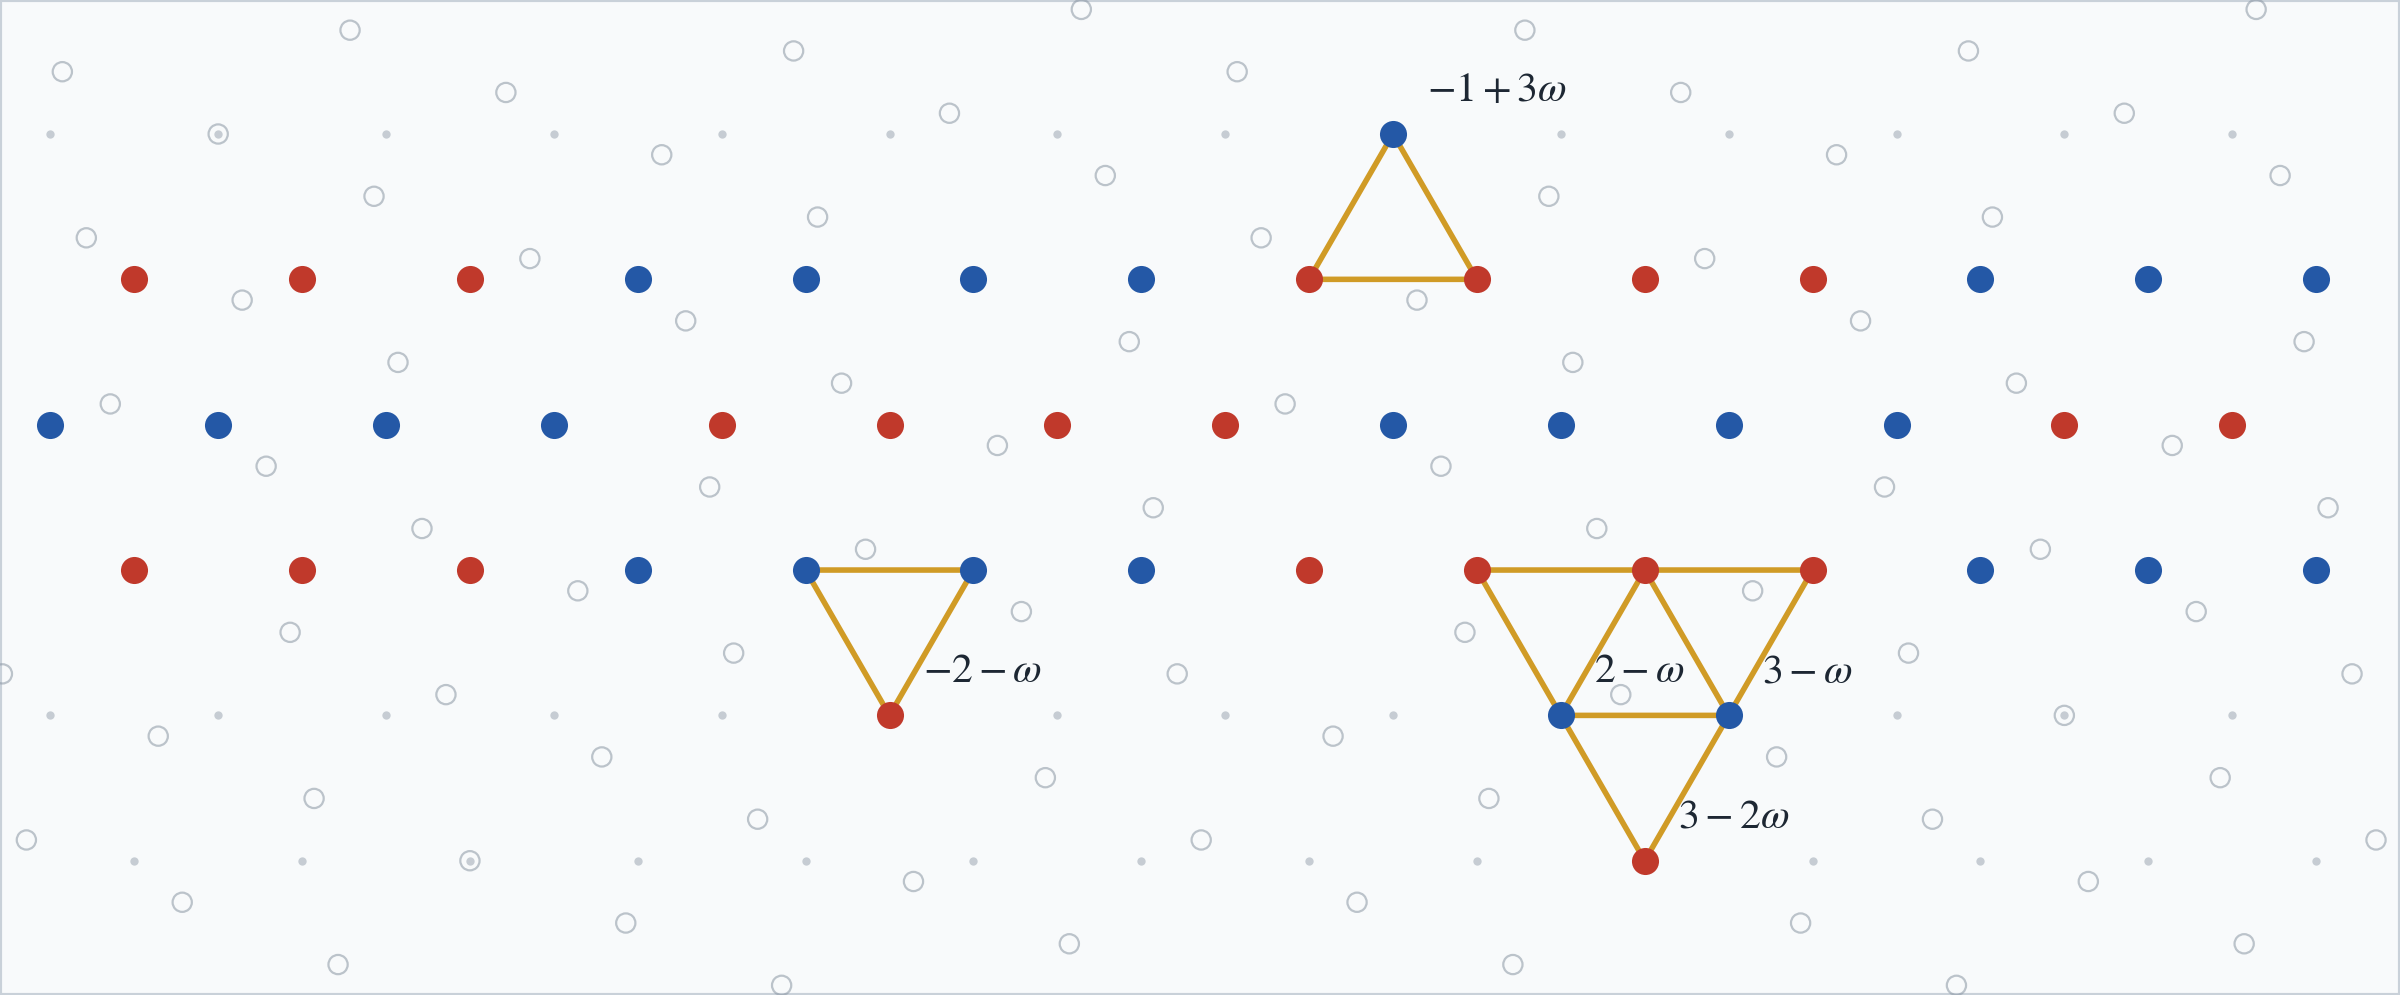
\includegraphics[width=\textwidth]{figures/ruleB_common.png}
\caption{The five deductions of Table~\ref{tab:common}, inside $\Lambda$ alone, from rows $0,1,2$.}\label{fig:common}\end{figure}

\emph{The cases.} By Theorem~\ref{thm:313} the long direction of $q\Lambda$ is $q\omega^j$ for some $j\in\{0,1,2\}$,
and by Corollary~\ref{cor:four} points of $q\Lambda$ four steps apart along it have opposite colours. In each case a
few more deductions end in a monochromatic forbidden triangle:

\paragraph{Case: the long direction of $q\Lambda$ is $q$.}
\begin{center}\small\begin{longtable}{rlll}\toprule & point & colour & because\\\midrule\endhead
1 & $q(2-2\omega)$ & red & four apart from $4+2\omega$ along $q$\\
2 & $q(1+\omega)$ & blue & four apart from $-2-\omega$ along $q$\\
3 & $q(2+\omega)$ & red & $T(1)$ with $-1+3\omega$, $q(1+\omega)$ (blue)\\
\bottomrule\end{longtable}\end{center}
\noindent\emph{Contradiction:} $q(2+\omega)$, $q(2-2\omega)$, $3-2\omega$ are all red and form $T(1,3,4)$.\par\medskip
\begin{figure}[h]\centering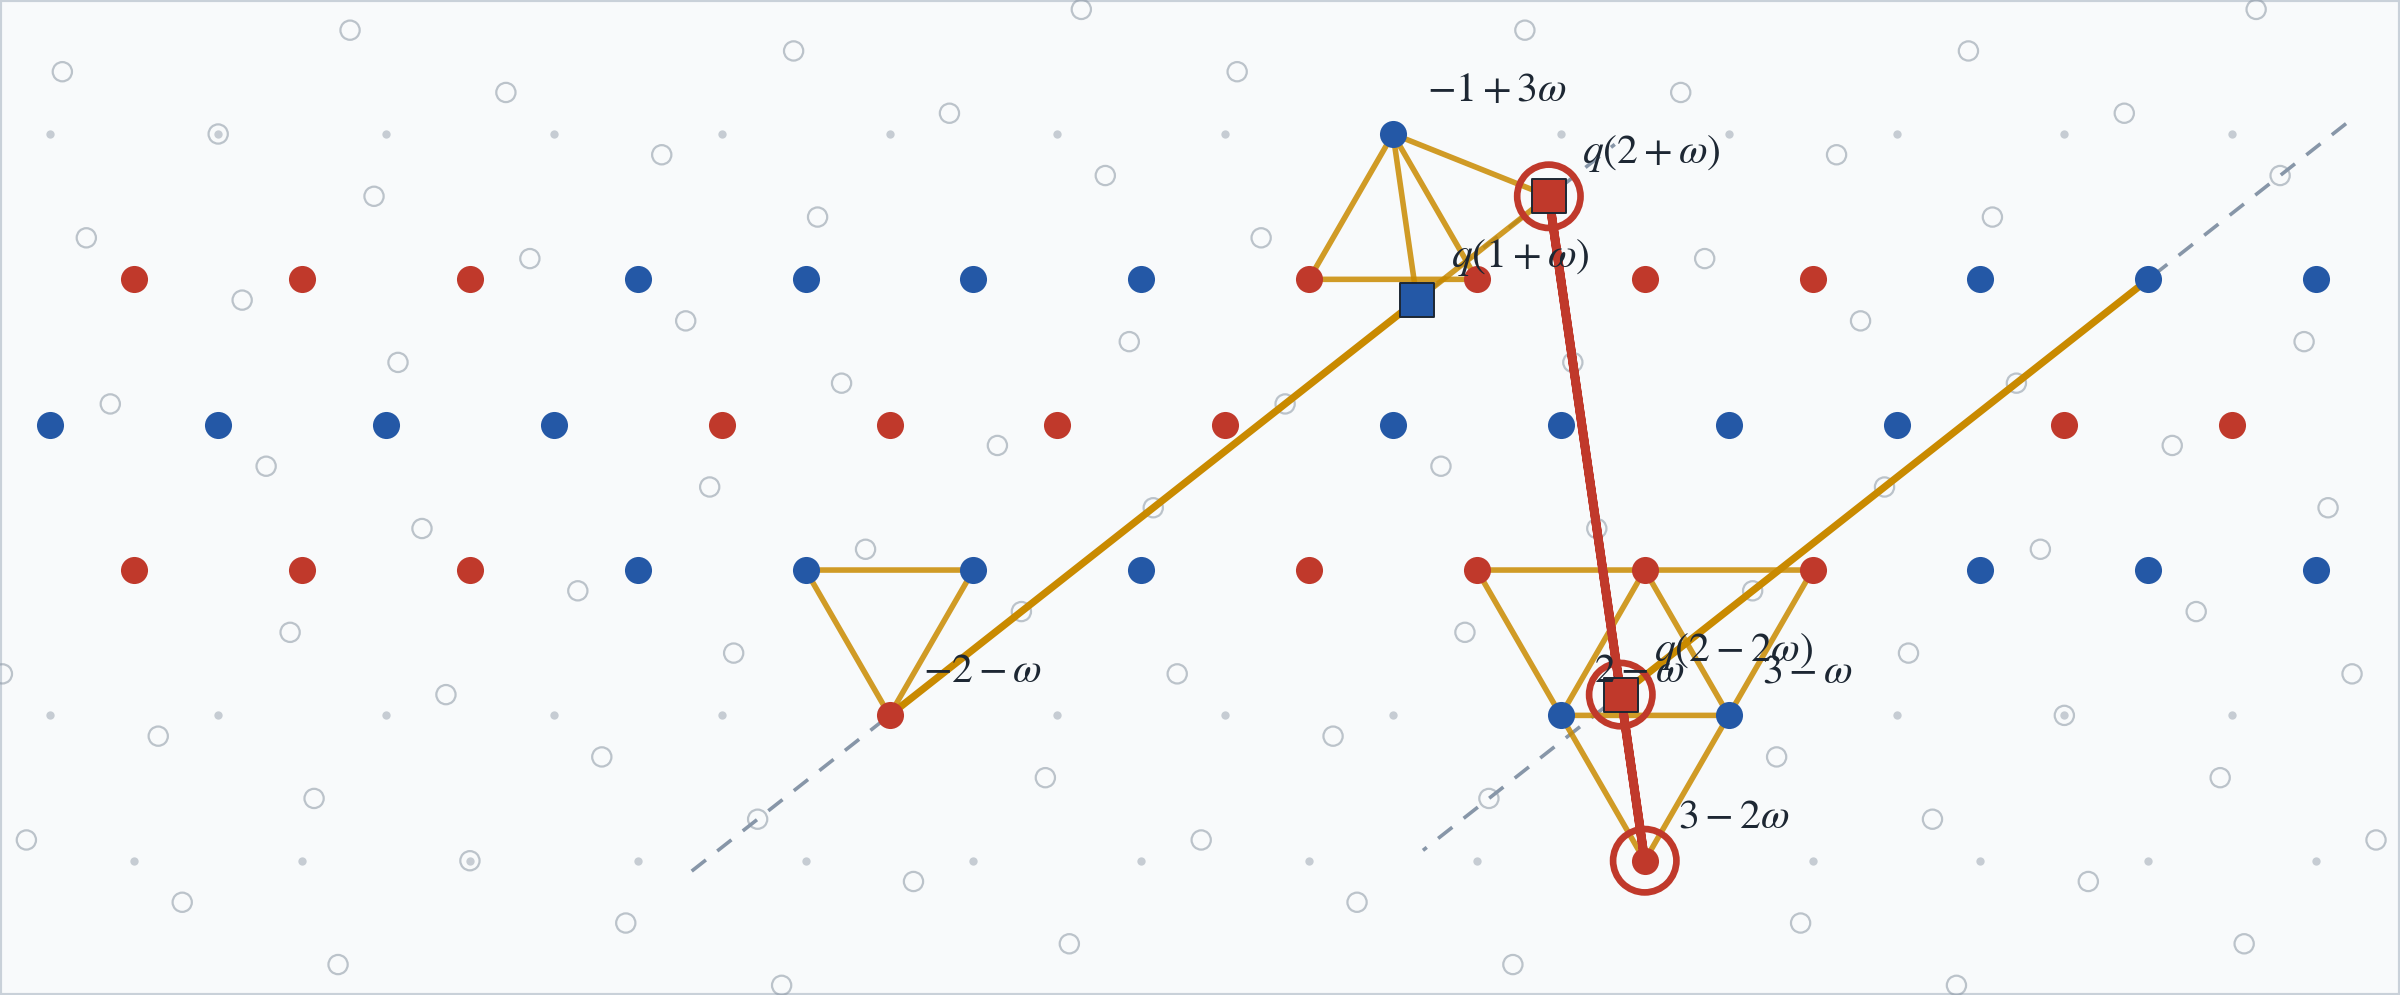
\includegraphics[width=\textwidth]{figures/ruleB_case0.png}\caption{Rule B, long direction $q$: every deduction of this case (amber), the four-apart steps along the dashed lines, and the contradiction (red).}\end{figure}
\paragraph{Case: the long direction of $q\Lambda$ is $q\omega$.}
\begin{center}\small\begin{longtable}{rlll}\toprule & point & colour & because\\\midrule\endhead
1 & $q(1-2\omega)$ & red & four apart from $-1+3\omega$ along $q\omega$\\
2 & $q(2+\omega)$ & blue & four apart from $3-2\omega$ along $q\omega$\\
3 & $q(-2+\omega)$ & blue & $T(1,3,4)$ with $q(1-2\omega)$, $3-2\omega$ (red)\\
4 & $-q$ & red & $T(1,3,4)$ with $-5+\omega$, $q(-2+\omega)$ (blue)\\
5 & $q(-1+\omega)$ & blue & $T(1)$ with $-q$, $0$ (red)\\
\bottomrule\end{longtable}\end{center}
\noindent\emph{Contradiction:} $q(-2+\omega)$, $q(-1+\omega)$, $q(2+\omega)$ are all blue and form $T(1,3,4)$.\par\medskip
\begin{figure}[h]\centering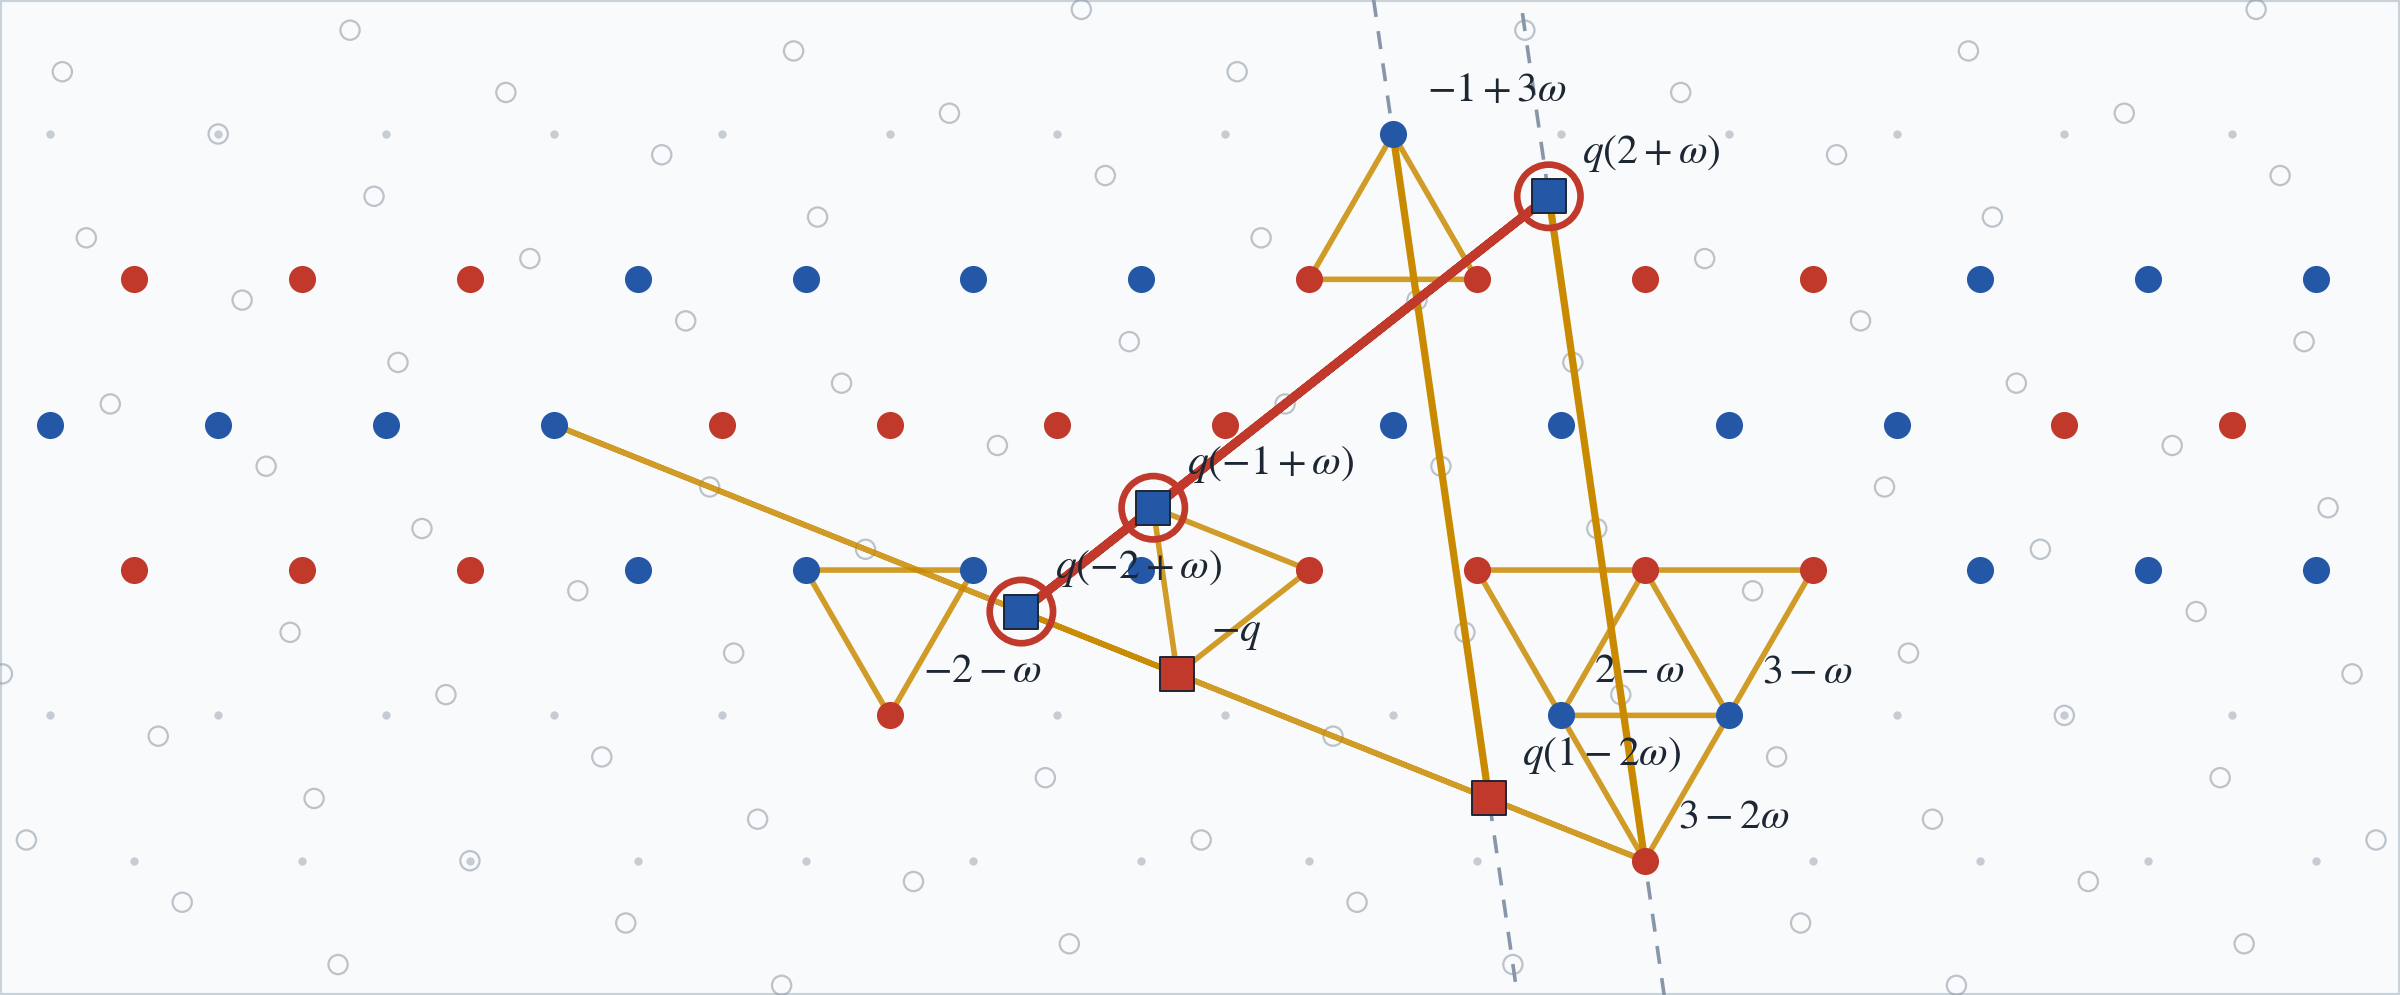
\includegraphics[width=\textwidth]{figures/ruleB_case1.png}\caption{Rule B, long direction $q\omega$: every deduction of this case (amber), the four-apart steps along the dashed lines, and the contradiction (red).}\end{figure}
\paragraph{Case: the long direction of $q\Lambda$ is $q\omega^2$.}
\begin{center}\small\begin{longtable}{rlll}\toprule & point & colour & because\\\midrule\endhead
1 & $q(-4+\omega)$ & blue & four apart from $-7$ along $q\omega^2$\\
2 & $-q$ & red & four apart from $-5+\omega$ along $q\omega^2$\\
3 & $q(-4+4\omega)$ & blue & four apart from $0$ along $q\omega^2$\\
4 & $q(-1+\omega)$ & blue & $T(1)$ with $-q$, $0$ (red)\\
\bottomrule\end{longtable}\end{center}
\noindent\emph{Contradiction:} $q(-4+4\omega)$, $q(-4+\omega)$, $q(-1+\omega)$ are all blue and form $T(3)$.\par\medskip
\begin{figure}[h]\centering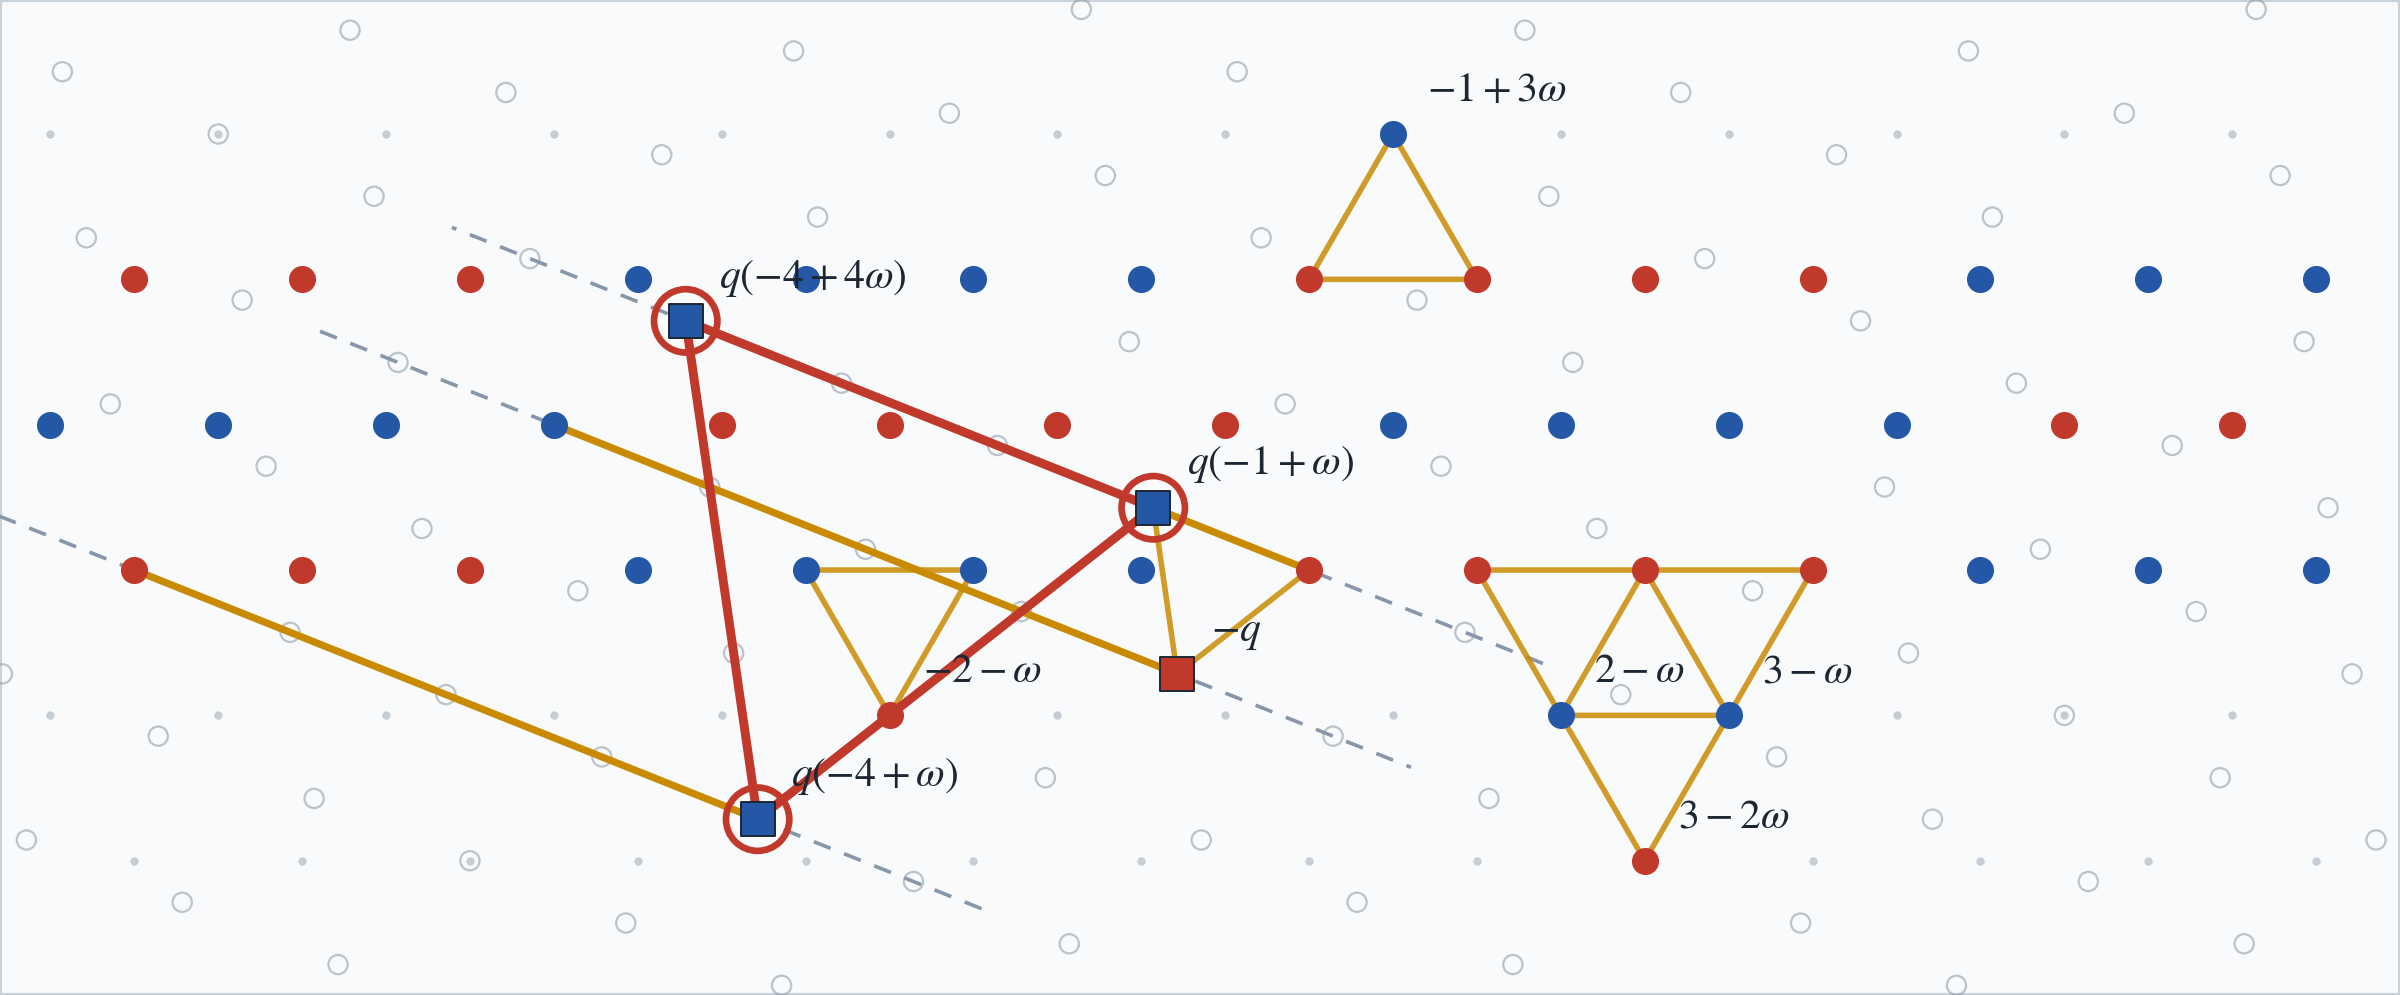
\includegraphics[width=\textwidth]{figures/ruleB_case2.png}\caption{Rule B, long direction $q\omega^2$: every deduction of this case (amber), the four-apart steps along the dashed lines, and the contradiction (red).}\end{figure}


All three directions are impossible, so $\Lambda$ has no turn.
\end{proof}



\section{Distance eight and the proof of Theorem~\ref{thm:main}}\label{sec:end}
\begin{proposition}\label{prop:d8}
In an admissible colouring, any two points at distance $8$ have the same colour.
\end{proposition}
\begin{proof}
Let $|p-p'|=8$ and take a unit triangular lattice in which $p'-p$ is eight unit steps. If its long direction is
parallel to $p'-p$, the row through $p,p'$ has period $8$. Otherwise choose coordinates in which the long direction
is $\omega$ times the old horizontal; since $8=\omega(8-8\omega)$, the endpoints have coordinates $(0,0)$ and $(8,-8)$
and colours $h(s_0)$ and $h(8+s_{-8})=h(s_{-8})$. By Rule B the eight steps between rows $-8$ and $0$ are all equal to
some $\delta\in\{4,5\}$, so $s_0-s_{-8}=8\delta\equiv0\pmod 8$. The other transverse direction is symmetric.
\end{proof}

\begin{proof}[Proof of Theorem~\ref{thm:main}]
Suppose $\chi$ is admissible and $|x-y|=1$. The circles of radius $8$ about $x$ and $y$ meet in a point $r$, and
Proposition~\ref{prop:d8} gives $\chi(x)=\chi(r)=\chi(y)$. So every unit equilateral triangle is monochromatic,
contradicting Lemma~\ref{lem:bridge}.
\end{proof}

\section{Verification}
The finite parts of Rule A and Rule B are recorded in certificates with standard-library verifiers. For Rule A the
verifier checks that every point lies in $\Lambda\cup q\Lambda$, re-derives all forbidden triangles from coordinates,
checks the symmetry statements and that the four cases' orbits cover all nine boundary colourings, and replays each
case with rule (F). For Rule B it checks Lemma~\ref{lem:pair} for all four pairs of steps and every deduction of
Table~\ref{tab:common} and of the three cases, each against exactly one rule. The tables in this
paper are generated from the certificates. Interactive walkthroughs of both rules accompany the code.

\begin{thebibliography}{9}
\bibitem{EGMRSS} P.~Erd\H{o}s, R.~L.~Graham, P.~Montgomery, B.~L.~Rothschild, J.~Spencer and E.~G.~Straus,
\emph{Euclidean Ramsey theorems.~III}, in: Infinite and Finite Sets, Colloq. Math. Soc. J\'anos Bolyai~10,
North-Holland, 1975, 559--583.
\bibitem{CMY24} G.~Currier, K.~Moore and C.~H.~Yip, \emph{Any two-coloring of the plane contains monochromatic
3-term arithmetic progressions}, Combinatorica \textbf{44} (2024), no.~6, 1367--1380.
\bibitem{Yan} A.~Yan, \emph{Monochromatic configurations in two-colored plane}, Bachelor's thesis, Charles University,
Prague, 2025.
\end{thebibliography}

\appendix
\section{Forcing tables for Rule A}\label{app:A}
Points are named in $\Lambda$ or as $q(m+n\omega)$. The row $-3,\dots,5$ is as in Lemma~\ref{lem:row}. In each case,
deductions are listed before the case split and in each subcase; each subcase ends in a contradiction.
\subsection*{Case 1: blue $-\omega$, $3-\omega$, $-1+\omega$, $2+\omega$}
\begin{figure}[h]\centering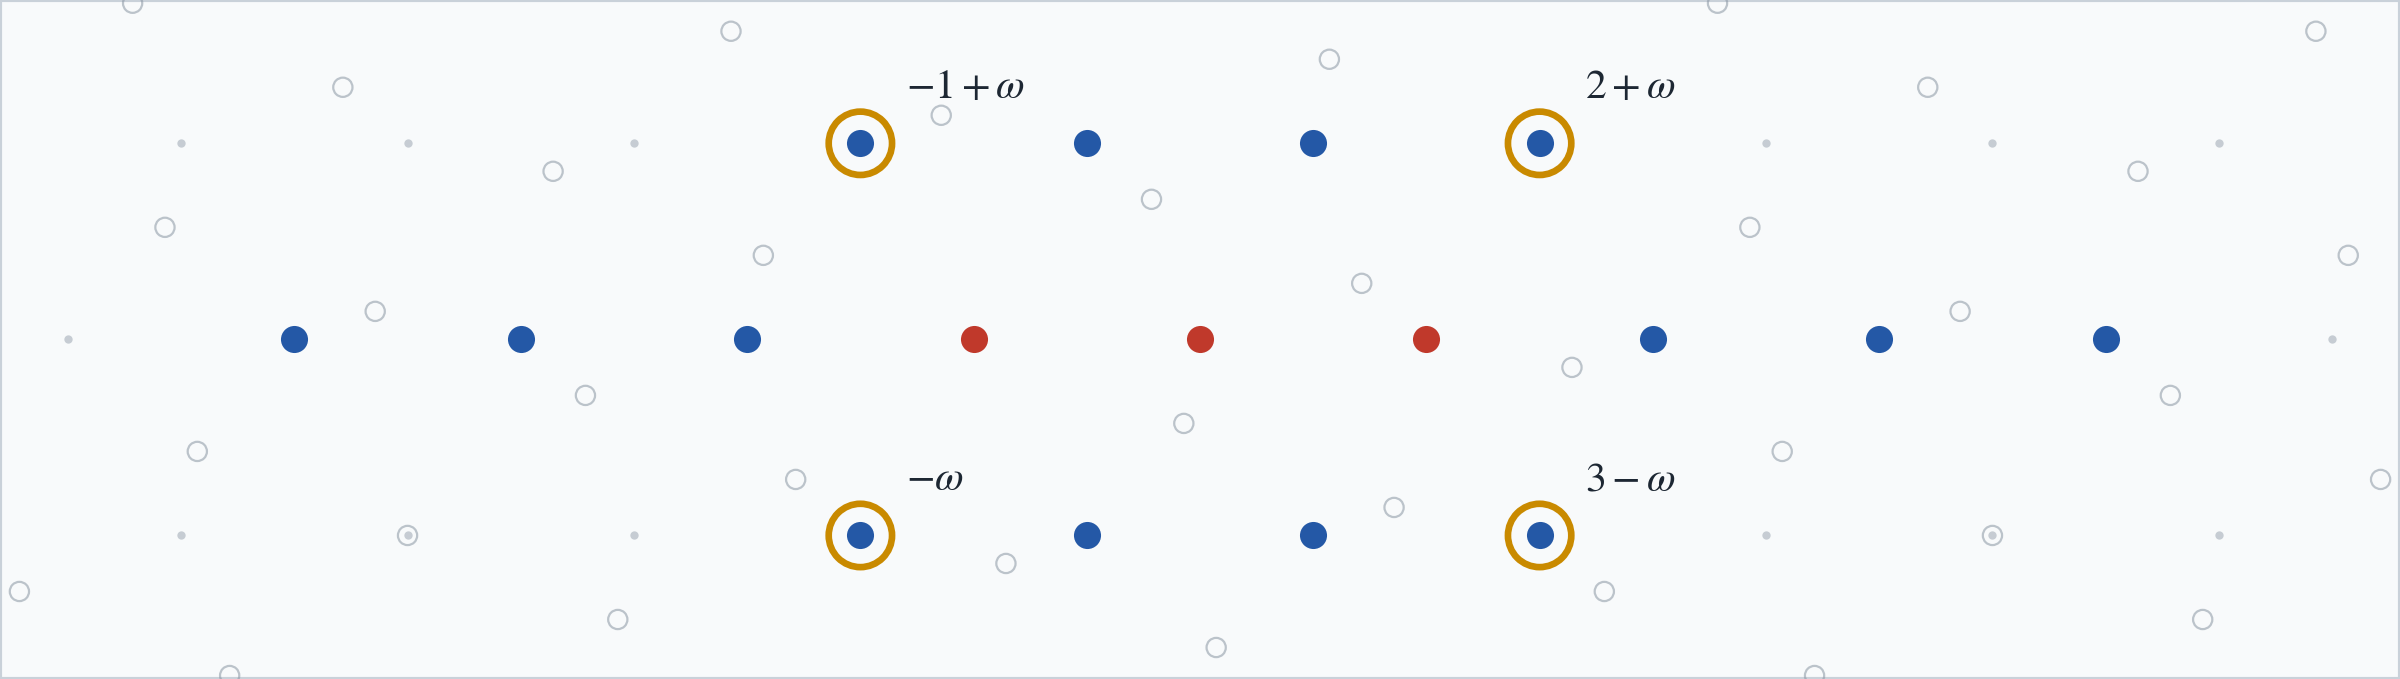
\includegraphics[width=\textwidth]{figures/ruleA_case1.png}\caption{Rule A, case 1: the row, the four forced points, and the boundary colouring of this case (ringed).}\end{figure}
\begin{center}\small\begin{longtable}{rlll}\toprule & point & colour & because\\\midrule\endhead
1 & $-1-\omega$ & red & $T(1)$ with $-2$, $-1$ (blue)\\
2 & $\omega$ & blue & $T(1)$ with $0$, $1$ (red)\\
3 & $1+\omega$ & blue & $T(1)$ with $1$, $2$ (red)\\
4 & $2-\omega$ & blue & $T(1)$ with $1$, $2$ (red)\\
5 & $7$ & red & $T(1,3,4)$ with $3$, $4$ (blue)\\
6 & $2\omega$ & red & $T(3)$ with $-\omega$, $3-\omega$ (blue)\\
7 & $3-2\omega$ & red & $T(1)$ with $2-\omega$, $3-\omega$ (blue)\\
8 & $-1+2\omega$ & red & $T(1)$ with $-1+\omega$, $\omega$ (blue)\\
9 & $1+2\omega$ & red & $T(1)$ with $1+\omega$, $2+\omega$ (blue)\\
10 & $-1+3\omega$ & blue & $T(1,3,4)$ with $-1-\omega$, $-1+2\omega$ (red)\\
11 & $4+2\omega$ & blue & $T(1,3,4)$ with $2\omega$, $1+2\omega$ (red)\\
\bottomrule\end{longtable}\end{center}
\paragraph{Subcase: $q(2+\omega)$ blue.}
\begin{center}\small\begin{longtable}{rlll}\toprule & point & colour & because\\\midrule\endhead
1 & $q(5-2\omega)$ & red & $T(1,3,4)$ with $-1+3\omega$, $q(2+\omega)$ (blue)\\
2 & $q(4-\omega)$ & blue & $T(1,3,4)$ with $q(5-2\omega)$, $7$ (red)\\
3 & $q(3\omega)$ & red & $T(1,3,4)$ with $-1+3\omega$, $q(4-\omega)$ (blue)\\
4 & $q(-\omega)$ & red & $T(1,3,4)$ with $2+\omega$, $q(4-\omega)$ (blue)\\
\bottomrule\end{longtable}\end{center}
\noindent\emph{Contradiction:} $q(3\omega)$, $0$, $q(-\omega)$ are all red and form $T(1,3,4)$.\par\medskip
\paragraph{Subcase: $q(2+\omega)$ red.}
\begin{center}\small\begin{longtable}{rlll}\toprule & point & colour & because\\\midrule\endhead
1 & $q(2)$ & blue & $T(1,3,4)$ with $q(2+\omega)$, $3-2\omega$ (red)\\
2 & $q(2-2\omega)$ & blue & $T(1,3,4)$ with $q(2+\omega)$, $3-2\omega$ (red)\\
3 & $q(3)$ & red & $T(1)$ with $q(2)$, $2+\omega$ (blue)\\
4 & $q(5-2\omega)$ & red & $T(1,3,4)$ with $q(2-2\omega)$, $4+2\omega$ (blue)\\
5 & $q(3\omega)$ & blue & $T(3)$ with $0$, $q(3)$ (red)\\
6 & $q(4-\omega)$ & blue & $T(1,3,4)$ with $q(5-2\omega)$, $7$ (red)\\
\bottomrule\end{longtable}\end{center}
\noindent\emph{Contradiction:} $q(3\omega)$, $-1+3\omega$, $q(4-\omega)$ are all blue and form $T(1,3,4)$.\par\medskip
\subsection*{Case 2: blue $3-\omega$, $-1+\omega$, $2+\omega$; red $-\omega$}
\begin{figure}[h]\centering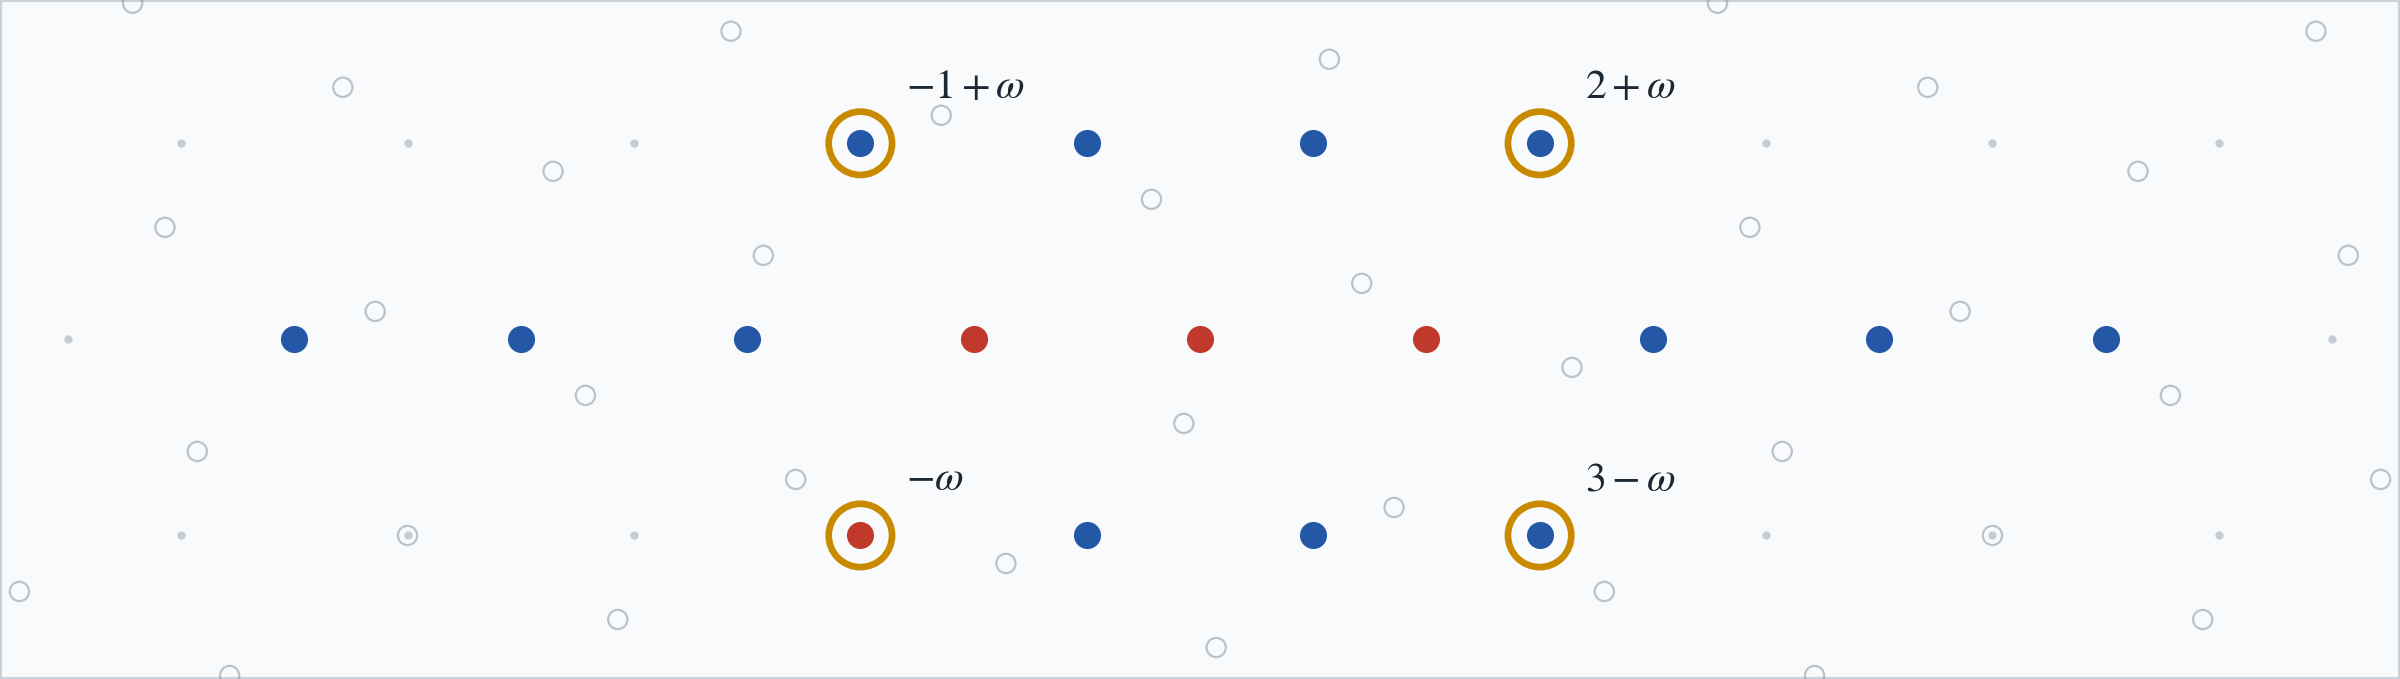
\includegraphics[width=\textwidth]{figures/ruleA_case2.png}\caption{Rule A, case 2: the row, the four forced points, and the boundary colouring of this case (ringed).}\end{figure}
\begin{center}\small\begin{longtable}{rlll}\toprule & point & colour & because\\\midrule\endhead
1 & $-1-\omega$ & red & $T(1)$ with $-2$, $-1$ (blue)\\
2 & $\omega$ & blue & $T(1)$ with $0$, $1$ (red)\\
3 & $1+\omega$ & blue & $T(1)$ with $1$, $2$ (red)\\
4 & $2-\omega$ & blue & $T(1)$ with $1$, $2$ (red)\\
5 & $7$ & red & $T(1,3,4)$ with $3$, $4$ (blue)\\
6 & $3-2\omega$ & red & $T(1)$ with $2-\omega$, $3-\omega$ (blue)\\
7 & $-1+2\omega$ & red & $T(1)$ with $-1+\omega$, $\omega$ (blue)\\
8 & $1+2\omega$ & red & $T(1)$ with $1+\omega$, $2+\omega$ (blue)\\
9 & $-1+3\omega$ & blue & $T(1,3,4)$ with $-1-\omega$, $-1+2\omega$ (red)\\
10 & $2\omega$ & red & $T(1)$ with $\omega$, $1+\omega$ (blue)\\
11 & $4+2\omega$ & blue & $T(1,3,4)$ with $2\omega$, $1+2\omega$ (red)\\
\bottomrule\end{longtable}\end{center}
\paragraph{Subcase: $q(2+\omega)$ blue.}
\begin{center}\small\begin{longtable}{rlll}\toprule & point & colour & because\\\midrule\endhead
1 & $q(5-2\omega)$ & red & $T(1,3,4)$ with $-1+3\omega$, $q(2+\omega)$ (blue)\\
2 & $q(4-\omega)$ & blue & $T(1,3,4)$ with $q(5-2\omega)$, $7$ (red)\\
3 & $q(3\omega)$ & red & $T(1,3,4)$ with $-1+3\omega$, $q(4-\omega)$ (blue)\\
4 & $q(-\omega)$ & red & $T(1,3,4)$ with $2+\omega$, $q(4-\omega)$ (blue)\\
\bottomrule\end{longtable}\end{center}
\noindent\emph{Contradiction:} $q(3\omega)$, $0$, $q(-\omega)$ are all red and form $T(1,3,4)$.\par\medskip
\paragraph{Subcase: $q(2+\omega)$ red.}
\begin{center}\small\begin{longtable}{rlll}\toprule & point & colour & because\\\midrule\endhead
1 & $q(2)$ & blue & $T(1,3,4)$ with $q(2+\omega)$, $3-2\omega$ (red)\\
2 & $q(2-2\omega)$ & blue & $T(1,3,4)$ with $q(2+\omega)$, $3-2\omega$ (red)\\
3 & $q(3)$ & red & $T(1)$ with $q(2)$, $2+\omega$ (blue)\\
4 & $q(5-2\omega)$ & red & $T(1,3,4)$ with $q(2-2\omega)$, $4+2\omega$ (blue)\\
5 & $q(3\omega)$ & blue & $T(3)$ with $0$, $q(3)$ (red)\\
6 & $q(4-\omega)$ & blue & $T(1,3,4)$ with $q(5-2\omega)$, $7$ (red)\\
\bottomrule\end{longtable}\end{center}
\noindent\emph{Contradiction:} $q(3\omega)$, $-1+3\omega$, $q(4-\omega)$ are all blue and form $T(1,3,4)$.\par\medskip
\subsection*{Case 3: blue $3-\omega$, $2+\omega$; red $-\omega$, $-1+\omega$}
\begin{figure}[h]\centering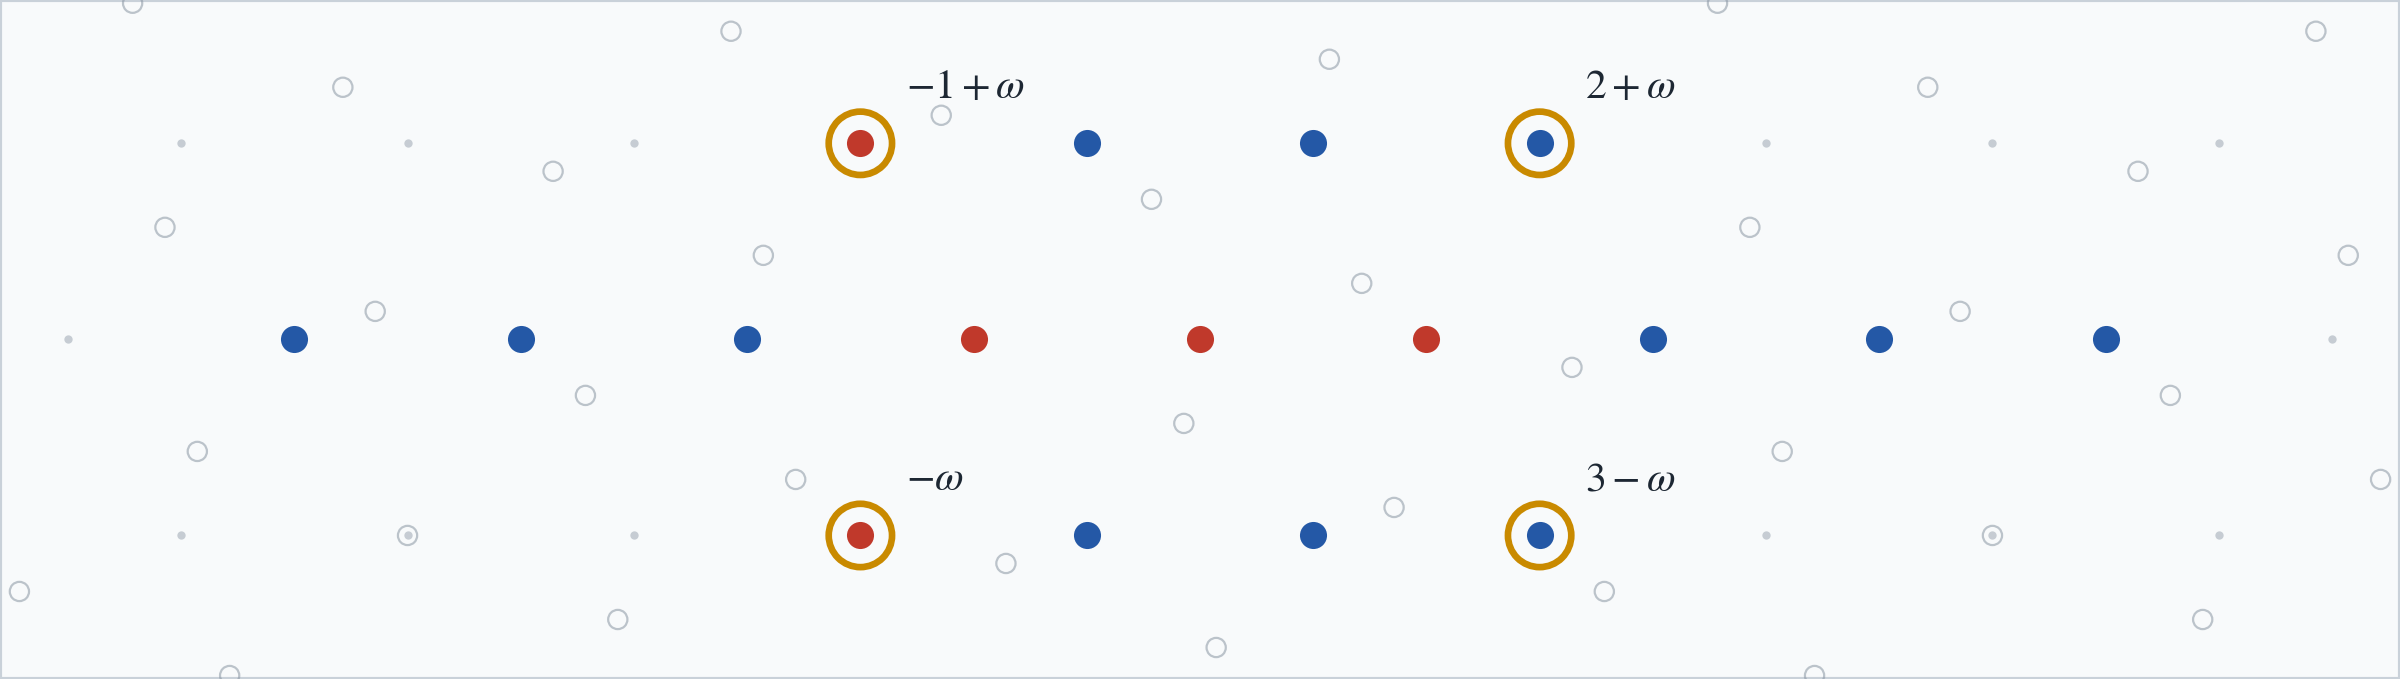
\includegraphics[width=\textwidth]{figures/ruleA_case3.png}\caption{Rule A, case 3: the row, the four forced points, and the boundary colouring of this case (ringed).}\end{figure}
\begin{center}\small\begin{longtable}{rlll}\toprule & point & colour & because\\\midrule\endhead
1 & $3-4\omega$ & red & $T(4)$ with $-1$, $3$ (blue)\\
2 & $\omega$ & blue & $T(1)$ with $-1+\omega$, $0$ (red)\\
3 & $1+\omega$ & blue & $T(1)$ with $1$, $2$ (red)\\
4 & $7$ & red & $T(1,3,4)$ with $3$, $4$ (blue)\\
5 & $5-\omega$ & red & $T(1)$ with $4$, $5$ (blue)\\
6 & $4-5\omega$ & blue & $T(1,3,4)$ with $-\omega$, $3-4\omega$ (red)\\
7 & $1+2\omega$ & red & $T(1)$ with $1+\omega$, $2+\omega$ (blue)\\
8 & $2\omega$ & red & $T(1)$ with $\omega$, $1+\omega$ (blue)\\
9 & $4+2\omega$ & blue & $T(1,3,4)$ with $2\omega$, $1+2\omega$ (red)\\
\bottomrule\end{longtable}\end{center}
\paragraph{Subcase: $q(5-5\omega)$ blue.}
\begin{center}\small\begin{longtable}{rlll}\toprule & point & colour & because\\\midrule\endhead
1 & $q(1-\omega)$ & red & $T(4)$ with $4-5\omega$, $q(5-5\omega)$ (blue)\\
2 & $q(4-5\omega)$ & red & $T(1,3,4)$ with $4-5\omega$, $q(5-5\omega)$ (blue)\\
3 & $q(-\omega)$ & blue & $T(1)$ with $0$, $q(1-\omega)$ (red)\\
4 & $q(4-\omega)$ & blue & $T(4)$ with $q(4-5\omega)$, $7$ (red)\\
\bottomrule\end{longtable}\end{center}
\noindent\emph{Contradiction:} $q(-\omega)$, $2+\omega$, $q(4-\omega)$ are all blue and form $T(1,3,4)$.\par\medskip
\paragraph{Subcase: $q(5-5\omega)$ red.}
\begin{center}\small\begin{longtable}{rlll}\toprule & point & colour & because\\\midrule\endhead
1 & $q(5-\omega)$ & blue & $T(1,3,4)$ with $5-\omega$, $q(5-5\omega)$ (red)\\
2 & $q(5-2\omega)$ & blue & $T(3)$ with $q(5-5\omega)$, $7$ (red)\\
\bottomrule\end{longtable}\end{center}
\noindent\emph{Contradiction:} $q(5-\omega)$, $q(5-2\omega)$, $4+2\omega$ are all blue and form $T(1)$.\par\medskip
\subsection*{Case 4: blue $-\omega$, $2+\omega$; red $3-\omega$, $-1+\omega$}
\begin{figure}[h]\centering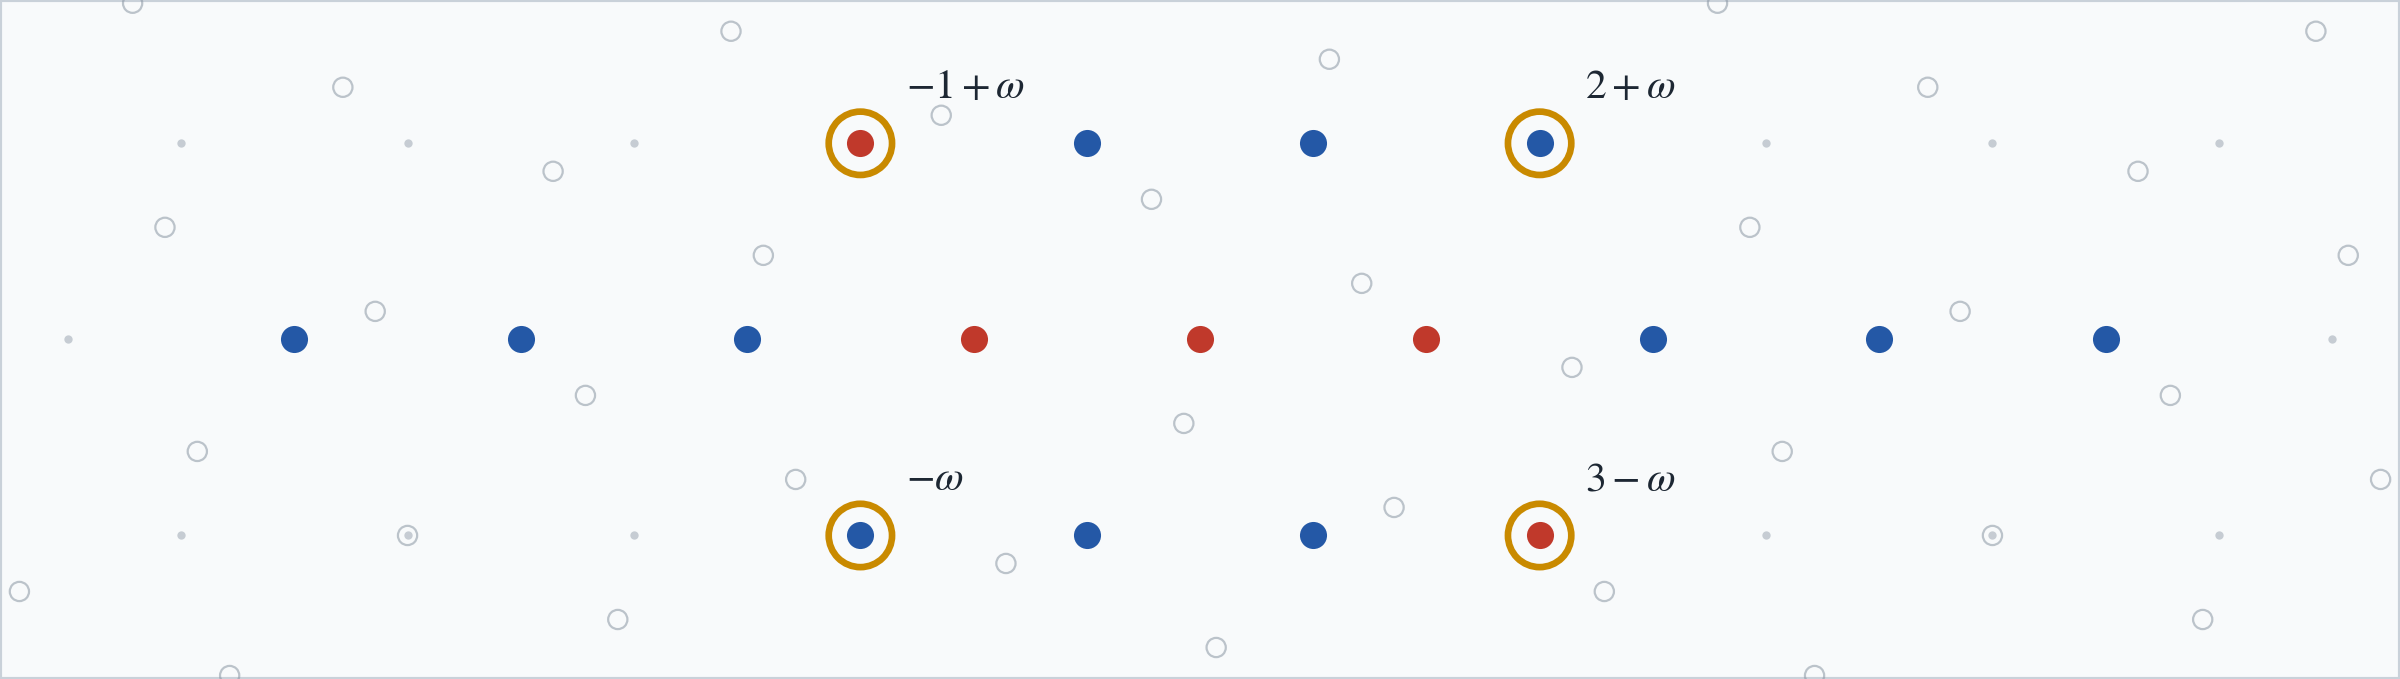
\includegraphics[width=\textwidth]{figures/ruleA_case4.png}\caption{Rule A, case 4: the row, the four forced points, and the boundary colouring of this case (ringed).}\end{figure}
\begin{center}\small\begin{longtable}{rlll}\toprule & point & colour & because\\\midrule\endhead
1 & $3-4\omega$ & red & $T(1,3,4)$ with $-1$, $-\omega$ (blue)\\
2 & $\omega$ & blue & $T(1)$ with $-1+\omega$, $0$ (red)\\
3 & $3-3\omega$ & blue & $T(1,3,4)$ with $-1+\omega$, $0$ (red)\\
4 & $1+\omega$ & blue & $T(1)$ with $1$, $2$ (red)\\
5 & $-1+3\omega$ & blue & $T(1,3,4)$ with $2$, $3-\omega$ (red)\\
6 & $6-4\omega$ & blue & $T(1,3,4)$ with $2$, $3-\omega$ (red)\\
7 & $7$ & red & $T(1,3,4)$ with $3$, $4$ (blue)\\
8 & $5-\omega$ & red & $T(1)$ with $4$, $5$ (blue)\\
9 & $1+2\omega$ & red & $T(1)$ with $1+\omega$, $2+\omega$ (blue)\\
10 & $2\omega$ & red & $T(1)$ with $\omega$, $1+\omega$ (blue)\\
11 & $4+2\omega$ & blue & $T(1,3,4)$ with $2\omega$, $1+2\omega$ (red)\\
\bottomrule\end{longtable}\end{center}
\paragraph{Subcase: $q(4-\omega)$ blue.}
\begin{center}\small\begin{longtable}{rlll}\toprule & point & colour & because\\\midrule\endhead
1 & $q(3\omega)$ & red & $T(1,3,4)$ with $-1+3\omega$, $q(4-\omega)$ (blue)\\
2 & $q(-\omega)$ & red & $T(1,3,4)$ with $2+\omega$, $q(4-\omega)$ (blue)\\
\bottomrule\end{longtable}\end{center}
\noindent\emph{Contradiction:} $q(3\omega)$, $0$, $q(-\omega)$ are all red and form $T(1,3,4)$.\par\medskip
\paragraph{Subcase: $q(4-\omega)$ red.}
\begin{center}\small\begin{longtable}{rlll}\toprule & point & colour & because\\\midrule\endhead
1 & $q(5-2\omega)$ & blue & $T(1,3,4)$ with $q(4-\omega)$, $7$ (red)\\
2 & $q(4-5\omega)$ & blue & $T(4)$ with $q(4-\omega)$, $7$ (red)\\
3 & $q(2+\omega)$ & red & $T(1,3,4)$ with $-1+3\omega$, $q(5-2\omega)$ (blue)\\
4 & $q(1-2\omega)$ & red & $T(4)$ with $-1+3\omega$, $q(5-2\omega)$ (blue)\\
5 & $q(2-2\omega)$ & red & $T(1,3,4)$ with $q(5-2\omega)$, $4+2\omega$ (blue)\\
6 & $q(5-\omega)$ & red & $T(1)$ with $q(5-2\omega)$, $4+2\omega$ (blue)\\
7 & $q(6-3\omega)$ & red & $T(1)$ with $q(5-2\omega)$, $4+2\omega$ (blue)\\
8 & $q(3-5\omega)$ & red & $T(1)$ with $q(4-5\omega)$, $6-4\omega$ (blue)\\
9 & $q(3)$ & blue & $T(1,3,4)$ with $q(2+\omega)$, $q(6-3\omega)$ (red)\\
10 & $q(1-\omega)$ & blue & $T(1)$ with $q(1-2\omega)$, $q(2-2\omega)$ (red)\\
11 & $q(5-5\omega)$ & blue & $T(1,3,4)$ with $q(5-\omega)$, $5-\omega$ (red)\\
12 & $q(3-4\omega)$ & red & $T(1,3,4)$ with $q(3)$, $2+\omega$ (blue)\\
13 & $4-5\omega$ & red & $T(4)$ with $q(1-\omega)$, $q(5-5\omega)$ (blue)\\
14 & $7-7\omega$ & blue & $T(1,3,4)$ with $q(3-4\omega)$, $q(3-5\omega)$ (red)\\
15 & $4-4\omega$ & blue & $T(1)$ with $3-4\omega$, $4-5\omega$ (red)\\
\bottomrule\end{longtable}\end{center}
\noindent\emph{Contradiction:} $3-3\omega$, $4-4\omega$, $7-7\omega$ are all blue and form $T(1,3,4)$.\par\medskip


\section{Rule A in two splits}\label{app:A2}
Here $3-\omega$ is blue, by $\sigma$ and Lemma~\ref{lem:boundary}, and the first split is at $q$.
\begin{center}\small\begin{longtable}{rlll}\toprule & point & colour & because\\\midrule\endhead
1 & $-6$ & red & $T(1,3,4)$ with $-3$, $-2$ (blue)\\
2 & $-3+\omega$ & red & $T(1)$ with $-3$, $-2$ (blue)\\
3 & $-2-\omega$ & red & $T(1)$ with $-3$, $-2$ (blue)\\
4 & $-5$ & red & $T(1,3,4)$ with $-2$, $-1$ (blue)\\
5 & $-2+\omega$ & red & $T(1)$ with $-2$, $-1$ (blue)\\
6 & $-1-\omega$ & red & $T(1)$ with $-2$, $-1$ (blue)\\
7 & $-1+4\omega$ & red & $T(4)$ with $-1$, $3$ (blue)\\
8 & $\omega$ & blue & $T(1)$ with $0$, $1$ (red)\\
9 & $1+\omega$ & blue & $T(1)$ with $1$, $2$ (red)\\
10 & $2-\omega$ & blue & $T(1)$ with $1$, $2$ (red)\\
11 & $3-2\omega$ & red & $T(1)$ with $2-\omega$, $3-\omega$ (blue)\\
12 & $3+\omega$ & red & $T(1)$ with $3$, $4$ (blue)\\
13 & $7$ & red & $T(1,3,4)$ with $3$, $4$ (blue)\\
14 & $4+\omega$ & red & $T(1)$ with $4$, $5$ (blue)\\
15 & $5-\omega$ & red & $T(1)$ with $4$, $5$ (blue)\\
16 & $-5-\omega$ & blue & $T(1)$ with $-6$, $-5$ (red)\\
17 & $-3+2\omega$ & blue & $T(1)$ with $-3+\omega$, $-2+\omega$ (red)\\
18 & $-1-2\omega$ & blue & $T(1)$ with $-2-\omega$, $-1-\omega$ (red)\\
19 & $2\omega$ & red & $T(1)$ with $\omega$, $1+\omega$ (blue)\\
20 & $3+2\omega$ & blue & $T(1,3,4)$ with $3-2\omega$, $3+\omega$ (red)\\
\bottomrule\end{longtable}\end{center}
\paragraph{Case: $q$ blue.}
\begin{center}\small\begin{longtable}{rlll}\toprule & point & colour & because\\\midrule\endhead
1 & $q(-3+4\omega)$ & red & $T(1,3,4)$ with $-3+2\omega$, $q$ (blue)\\
2 & $q(1+3\omega)$ & red & $T(3)$ with $-3+2\omega$, $q$ (blue)\\
3 & $q(2-\omega)$ & red & $T(1,3,4)$ with $-3+2\omega$, $q$ (blue)\\
4 & $q(\omega)$ & blue & $T(3)$ with $q(-3+4\omega)$, $-2-\omega$ (red)\\
5 & $q(5-\omega)$ & blue & $T(3)$ with $q(2-\omega)$, $5-\omega$ (red)\\
6 & $q(4-3\omega)$ & red & $T(1,3,4)$ with $q(\omega)$, $q$ (blue)\\
7 & $q(5-3\omega)$ & blue & $T(1)$ with $q(4-3\omega)$, $5-\omega$ (red)\\
\bottomrule\end{longtable}\end{center}
\paragraph{Subcase: $q(4-\omega)$ blue.}
\begin{center}\small\begin{longtable}{rlll}\toprule & point & colour & because\\\midrule\endhead
1 & $q(1-\omega)$ & red & $T(1,3,4)$ with $q(4-\omega)$, $q(5-\omega)$ (blue)\\
2 & $q(-3+3\omega)$ & blue & $T(4)$ with $q(1+3\omega)$, $q(1-\omega)$ (red)\\
3 & $q(-2-\omega)$ & blue & $T(1,3,4)$ with $q(1-\omega)$, $q(2-\omega)$ (red)\\
4 & $q(-\omega)$ & blue & $T(1)$ with $0$, $q(1-\omega)$ (red)\\
5 & $q(2-2\omega)$ & blue & $T(1)$ with $q(1-\omega)$, $q(2-\omega)$ (red)\\
6 & $q(-6+3\omega)$ & red & $T(1,3,4)$ with $q(-3+3\omega)$, $-3+2\omega$ (blue)\\
7 & $2+\omega$ & red & $T(1,3,4)$ with $q(-\omega)$, $q(4-\omega)$ (blue)\\
8 & $-1+\omega$ & blue & $T(1,3,4)$ with $-2+\omega$, $2+\omega$ (red)\\
9 & $q(-1-\omega)$ & blue & $T(1,3,4)$ with $q(2-\omega)$, $2+\omega$ (red)\\
10 & $q(3-2\omega)$ & blue & $T(1)$ with $q(2-\omega)$, $2+\omega$ (red)\\
11 & $-4+\omega$ & red & $T(3)$ with $-1-2\omega$, $-1+\omega$ (blue)\\
12 & $1-3\omega$ & red & $T(1)$ with $q(-2-\omega)$, $q(-1-\omega)$ (blue)\\
13 & $4+2\omega$ & red & $T(1,3,4)$ with $q(2-2\omega)$, $q(3-2\omega)$ (blue)\\
14 & $-7+\omega$ & blue & $T(1,3,4)$ with $-4+\omega$, $-3+\omega$ (red)\\
15 & $-3-3\omega$ & blue & $T(4)$ with $-3+\omega$, $1-3\omega$ (red)\\
16 & $1+2\omega$ & blue & $T(1,3,4)$ with $2\omega$, $4+2\omega$ (red)\\
17 & $-4-2\omega$ & red & $T(1,3,4)$ with $-7+\omega$, $-3-3\omega$ (blue)\\
18 & $-2+2\omega$ & red & $T(1,3,4)$ with $-3+2\omega$, $1+2\omega$ (blue)\\
19 & $q(-6+6\omega)$ & blue & $T(1,3,4)$ with $q(-6+3\omega)$, $-4-2\omega$ (red)\\
20 & $-5+2\omega$ & blue & $T(3)$ with $-2-\omega$, $-2+2\omega$ (red)\\
21 & $-8+3\omega$ & red & $T(1,3,4)$ with $q(-6+6\omega)$, $q(-3+3\omega)$ (blue)\\
22 & $-5+3\omega$ & red & $T(1,3,4)$ with $-5-\omega$, $-5+2\omega$ (blue)\\
\bottomrule\end{longtable}\end{center}
\noindent\emph{Contradiction:} $-8+3\omega$, $-5$, $-5+3\omega$ are all red and form $T(3)$.\par\medskip
\paragraph{Subcase: $q(4-\omega)$ red.}
\begin{center}\small\begin{longtable}{rlll}\toprule & point & colour & because\\\midrule\endhead
1 & $q(5-2\omega)$ & blue & $T(1,3,4)$ with $q(4-\omega)$, $7$ (red)\\
2 & $4+2\omega$ & red & $T(1)$ with $q(5-\omega)$, $q(5-2\omega)$ (blue)\\
3 & $q(4-2\omega)$ & red & $T(1)$ with $q(5-2\omega)$, $q(5-3\omega)$ (blue)\\
4 & $1+2\omega$ & blue & $T(1,3,4)$ with $2\omega$, $4+2\omega$ (red)\\
5 & $2+\omega$ & blue & $T(1)$ with $q(4-\omega)$, $q(4-2\omega)$ (red)\\
\bottomrule\end{longtable}\end{center}
\noindent\emph{Contradiction:} $1+\omega$, $1+2\omega$, $2+\omega$ are all blue and form $T(1)$.\par\medskip
\paragraph{Case: $q$ red.}
\begin{center}\small\begin{longtable}{rlll}\toprule & point & colour & because\\\midrule\endhead
1 & $q(\omega)$ & blue & $T(1)$ with $0$, $q$ (red)\\
2 & $q(1-\omega)$ & blue & $T(1)$ with $0$, $q$ (red)\\
3 & $q(2-\omega)$ & blue & $T(1,3,4)$ with $q$, $5-\omega$ (red)\\
4 & $q(4-3\omega)$ & blue & $T(1,3,4)$ with $q$, $5-\omega$ (red)\\
5 & $1+4\omega$ & red & $T(4)$ with $q(\omega)$, $q(4-3\omega)$ (blue)\\
6 & $q(2-2\omega)$ & red & $T(1)$ with $q(1-\omega)$, $q(2-\omega)$ (blue)\\
7 & $q(-1+2\omega)$ & red & $T(1,3,4)$ with $-3+2\omega$, $q(2-\omega)$ (blue)\\
8 & $q(2+3\omega)$ & red & $T(4)$ with $-3+2\omega$, $q(2-\omega)$ (blue)\\
9 & $-3+4\omega$ & blue & $T(4)$ with $1$, $1+4\omega$ (red)\\
10 & $5\omega$ & blue & $T(1,3,4)$ with $1+4\omega$, $4+\omega$ (red)\\
11 & $q(1-2\omega)$ & blue & $T(1)$ with $q(2-2\omega)$, $3-2\omega$ (red)\\
12 & $-4+5\omega$ & red & $T(1,3,4)$ with $-3+4\omega$, $\omega$ (blue)\\
13 & $-1+6\omega$ & red & $T(1,3,4)$ with $5\omega$, $3+2\omega$ (blue)\\
14 & $-1+3\omega$ & red & $T(1,3,4)$ with $q(1-\omega)$, $q(1-2\omega)$ (blue)\\
15 & $q(-\omega)$ & red & $T(1)$ with $q(1-\omega)$, $q(1-2\omega)$ (blue)\\
16 & $q(-4+5\omega)$ & blue & $T(3)$ with $-4+5\omega$, $q(-1+2\omega)$ (red)\\
17 & $-1+7\omega$ & blue & $T(1,3,4)$ with $-1+3\omega$, $-1+6\omega$ (red)\\
18 & $q(3\omega)$ & blue & $T(1,3,4)$ with $0$, $q(-\omega)$ (red)\\
19 & $q(-3+4\omega)$ & red & $T(1,3,4)$ with $q(-4+5\omega)$, $q(\omega)$ (blue)\\
20 & $q(5\omega)$ & red & $T(4)$ with $q(-4+5\omega)$, $q(\omega)$ (blue)\\
21 & $q(1+4\omega)$ & blue & $T(4)$ with $q(-3+4\omega)$, $q$ (red)\\
22 & $q(4\omega)$ & blue & $T(1)$ with $-4+5\omega$, $q(5\omega)$ (red)\\
23 & $q(1+3\omega)$ & red & $T(1)$ with $q(4\omega)$, $q(1+4\omega)$ (blue)\\
24 & $-5+8\omega$ & red & $T(1,3,4)$ with $q(4\omega)$, $q(3\omega)$ (blue)\\
25 & $7\omega$ & blue & $T(1,3,4)$ with $q(1+3\omega)$, $q(2+3\omega)$ (red)\\
26 & $-4+7\omega$ & blue & $T(1,3,4)$ with $-5+8\omega$, $-1+4\omega$ (red)\\
\bottomrule\end{longtable}\end{center}
\noindent\emph{Contradiction:} $-4+7\omega$, $-1+7\omega$, $7\omega$ are all blue and form $T(1,3,4)$.\par\medskip

\end{document}
